\documentclass[b5paper,opensource]{./template/qyxf-book}
%注意,我修改了模板里的\solve,使其后文字首行缩进两字符
\usepackage{subcaption}
\usepackage{draftwatermark}
\usepackage{fontawesome5}
\SetWatermarkText{钱院学辅}
\SetWatermarkLightness{0.92}
\SetWatermarkScale{0.9}

\usepackage{siunitx}%输入角度
\usepackage{color}
\renewcommand{\thefootnote}{\color{red}\arabic{footnote}}%更改脚注格式
\usepackage[version=4]{mhchem}%写化学式
\newcommand{\RNum}[1]{\uppercase\expandafter{\romannumeral #1\relax}}%罗马数字
\newenvironment{mymathfrac}[2]{\left.\raise0.5ex\hbox{$#1$}\! \big\left/ \! \lower0.5ex\hbox{$#2$}\right.}%长斜分数线环境
%公式按照题目标号,不知道为啥编译不了,只能手动添加到各章
%\makeatletter
%\@addtoreset{equation}{exercise}
%\makeatother
%\renewcommand{\theequation}{(\arabic{section}.\arabic{equation})}

\graphicspath{{pics/}}%图片全部保存在pics文件夹



\title{大学物理题解(下)}
\subtitle{Key to University Physics: Part \RNum{2}}
\author{钱院学辅大物编写小组}
\typo{钱院学辅排版组}
\date{2019 年 12 月  日}
\version{v1.0}
\sourcepage{\url{https://github.com/qyxf/BookHub/}}

\begin{document}
	
\maketitle
\pagestyle{plain}
\chapter*{前言}
大学物理(University Physics)是本校理工科学生在大一、大二年级所要学习的一门自然科学
基础课程。这门课程课时较多、内容丰富,相关的练习题与考试题则尤显花样繁多,充分考验着每一个
学生对相关知识的掌握程度与应用能力。从掌握知识的角度来说,多做、精做大物习题是学好这门
课程的必经之路;从备考、应试的角度来说,若不熟练掌握各类大物习题的思路与解法,而仅依靠课内所
学到的基本知识点,则不可能在考试中取得令人满意的成绩。因此,熟练掌握本课程相关练习题的
解题技巧,是非常必要的。

“不积跬步,无以至千里。”一份可靠的题解,需要经过多次的改进才可望真正铸造出来。虽然这份题解的确可谓“精心制作”,但笔误、错漏等在所难免,特别需要各位使用者帮助我们指正。如您在参考的过程中发现有任何错误
之处,欢迎您通过下面的方式联系我们,帮助我们改进这份题解:
%\begin{itemize}
	%\item \faGithub ~~ GitHub平台论坛(\textbf{推荐,但需要注册}):\url{https://github.com/qyxf/BookHub/issues}
	%\item \faInternetExplorer ~~ 钱院学辅信息发布站:\url{https://qyxf.github.io}
	%\item \faEnvelopeOpen ~~ 钱院学辅邮箱:\texttt{qianxiaofu.mail@qq.com}
	%\item \faQq ~~ 钱院学辅官方答疑墙:~~\textbf{钱小辅}~~206713407
%\end{itemize}

作为钱院学辅出品的第一份“重量级”作品,希望它能够带给每一位同学最好的体验!

\begin{flushright}
	钱院学辅大物编写小组\\
	2019 年 12 月 7 日
\end{flushright}
\vspace{1.0cm}
\begin{figure}[!h]
	\centering
	\begin{minipage}[c]{0.5\textwidth}
		\centering
		
\includegraphics[scale=0.5]{./template/qrcode2.png}
	\end{minipage}%
	\begin{minipage}[c]{0.5\textwidth}
		\centering
		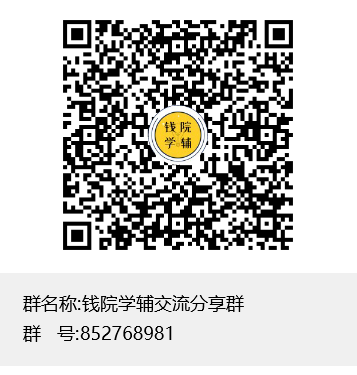
\includegraphics[scale=0.5]{./template/new_group.png}
	\end{minipage}
\end{figure}
%需要交流分享群二维码


\cleardoublepage
\tableofcontents

\setcounter{chapter}{10}

\chapter{热力学基础}
\section{选择题}
\exercise C

\solve 
等体加热内能增大,A错;

等温过程内能不变,$\Delta E = 0$,$Q+A>0$,$Q<0$,B错;

由$PV=nRT$,$V\uparrow$,则$T\uparrow$,则$\Delta E>0$,又$A<0$,则$Q>0$,C正确;

绝热压缩,$A>0$,$Q=0$,则$\delta E>0$,D错。

\exercise A

\solve 
由容积不变知为等体过程,则${Q_V} = \nu {C_V}({T_2} - {T_1})$,$H_2$为双原子分子,${C_V} = \frac{5}{2}R,$ \ce{NH3}为多原子分子,$C_V=3R$(本章未提及),则A正确。


\exercise B

\solve 由图中ab及cd围成面积知$\Delta {E_{ab}} = \Delta {E_{cd}}$,$A_{ab} < {A_{cd}}$,由$\Delta E = Q + A$知$Q_{ab} > {Q_{cd}}$,又${Q_{ab}}= 0$,所以${A_{cb}} < 0$,即$C < 0$,故选B。


\exercise D

\solve 等温:$\delta T=0$

等压:由$PV=nRT$,$\frac{V_2}{V_1}=\frac{T_2}{T_1}\Rightarrow \left|\delta T\right|=T_1$

绝热:由$TV^\gamma=C_2$知$(\frac{V_1}{V_2})^{\gamma-1}=\frac{T_2}{T_1}\Rightarrow \left|\delta T\right|=\left|[1-(\frac{1}{2})^{\gamma-1}]T_1\right|$

则选D。

\exercise D

\solve 绝热线与等温线只有一个交点,A错;

由$PV=nRT$,两者内能变化量相同,但做功不同,则吸热量不同,B错;

曲线下围成面积不同,C错;

由$PV=nRT$,D对。

\exercise D

\solve 等压过程,系统对外做功$A=\nu R(T_2-T_1)$,吸热$Q_P=\nu C_P(T_2-T_1)$,则$\frac{W}{Q}=\frac{A}{Q_P}=\frac{R}{C_P}=\frac{1}{1+\frac{5}{2}}=\frac{2}{7}$

故选D。

\exercise C

\solve $\eta=1-\frac{T_1}{T_2}$,易知BCC'和ADD'分别为等温线,则$\eta_1=\eta_2$;
由图,BCD下面积小于BCD',则$W_1<W_2$,故选C。

\exercise C

\solve 体积增大,则W>0;

$T_a=\frac{2p_1V_1}{nR}=T_b$,则$\Delta E=0$,故选C。

\exercise B

\solve A错,绝热斜率应该比等温线绝对值大;

B是合理的;

C、D选项,绝热线不能相交;

故选B。

\exercise D

\solve 假设可行,则$\eta=1000/1600=62.5\%$;

而由卡诺循环,$\eta=1-\frac{T_2}{T_1}=25\%$,故选D。

\section{计算题}
\exercise $\frac{1}{2}(\frac{C}{V_1^2}-\frac{C}{V_2^2})$或$\frac{1}{2}(P_1V_1-P_2V_2)$\qquad 减少\qquad 放热

\solve $W = \int_{{V_1}}^{{V_2}} {p\di{V} = } \int_{V_1}^{V_2}{\frac{C}{{{V^3}}}\di{V}=}- \frac{1}{2}(\frac{C}{{{V_2}^2}}-\frac{C}{{{V_1}^2}})=\frac{1}{2}(P_1V_1-P_2V_2)$

由$PV = nRT,P{V^3} = C$得$T=\frac{C}{nRV^2}$,V增加,T减少,则气体内能减少

$\Delta E = \nu {C_V}({T_2}-{T_1})= \frac{{{C_V}({p_2}{V_2} - {p_1}{V_1})}}{R} = \frac{C_V}{R}(\frac{C}{V_2^2}-\frac{C}{V_1^2})$

$\Delta Q = \Delta  + A = (\frac{C_V}{R} - \frac{1}{2})(\frac{C}{V_2^2} - \frac{C}{V_1^2}) < 0$

所以放热。

\exercise 不重合\qquad$\gamma$不同\qquad 不重合

\solve
$\gamma$不同,则其函数型$pV^\gamma=C$不同。

\exercise 500\qquad700

\solve 
等压过程中,$A=p\Delta V=\nu \Delta T$,单原子分子$C_{P1}=\frac{5}{2}R$

$Q_1=\nu C_{P1} \Delta T=\dfrac{5}{2}A=500\mathrm{J}$

$Q_2=\nu C_{P2} \Delta T=\dfrac{7}{2}A=700\mathrm{J}$

\exercise 温度\qquad 过程\qquad 做功\qquad 传递热量

\exercise 2/3\qquad$2S_1$

\solve
$\eta =1-\frac{T_0}{3T_0}=\frac{2}{3}$

$W=\frac{S_1}{1-\eta}-S_1=2S_1$

\exercise 1/3\qquad200J

\solve
$\eta =1-\frac{T_2}{T_1}=\frac{1}{3}$

$W=\frac{T_2}{T_1-T_2}=2\mathrm{J}$

$A=\frac{Q_2}{W}=200\mathrm{J}$

\exercise =\qquad >

\solve 两种气体对外做功即为abcda围成的面积,相等。

$\eta=\frac{W}{Q},W$相同,由$pV=nRT$知温度变化量也相同;

ab过程为等压过程,且$C_{\text{\RNum{1}}}<C_\text{\RNum{2}}$,则$Q_{\text{\RNum{1}}}<Q_{\text{\RNum{2}}}$,则有$\eta_{\text{\RNum{1}}}>\eta_{\text{\RNum{2}}}$

\exercise $\frac{1}{2}p_0V_0\qquad 9p_0V_0$

\solve W即为1\to2\to3\to1围成的面积,易得$W=\frac{1}{2}p_0V_0$

$\Delta E=\nu C_V\Delta T=\frac{3C_Vp_0V_0}{R}=\frac{15p_0V_0}{2}$

对外做功为1\to2下的面积,即$A=\frac{3p_0V_0}{2}$,则$Q=\Delta E+A=9p_0V_0$

\exercise 3R

\solve
%gxf对原解答做了改动
$A=\frac{3p_1V_1}{2}$,$\Delta T=\frac{\Delta(PV)}{\nu R}=\frac{3p_1V_1}{R}$

$\Delta E=\nu C_V\Delta T=\frac{15p_1V_1}{2}$

$Q=\Delta E+A=9p_1V_1$

\therefore$C=\frac{Q}{\Delta T}=3R$

\exercise 40J\qquad 120J

\solve 由EBCE循环系统对外做功70J,EDAE过程外界对系统做功30J,则一次循环过程系统对外做净功40J;

由于AEB为绝热过程,则$Q_{EAB}=0$,由$Q=\Delta E+A$知:

$W+\Delta E=Q_{BC}+Q_{CED}+Q_{DA}$

由于理想气体一次循环中的内能不变,则$\Delta=500$,则有$40=-30+Q_{CED}-50$,则
$Q_{CED}=120\mathrm{J}$

又因为CED为等体过程,则$A_{CED}=0,\Delta E=120\mathrm{J}$.

\section{解答题}

\exercise

\solve 由\[Q = \Delta E + A\]

知\[\eta=1-\frac{{\Delta {E_{BC}} + {A_{BC}}}}{{\Delta {E_{DA}} + A{  _{DA}}}}\]
\[{A_{BC}}=-\frac{1}{2}({p_B} + {p_C})({V_B} - {V_C})\]
\[\Delta {E_{BC}} = \nu {C_V}({T_C} - {T_B}) = \frac{{{C_V}({p_C}{V_C} - {p_B}{V_B})}}{R} = \frac{1}{{\gamma  - 1}}({p_C}{V_C} - {p_B}{V_B})\]
\[ \Rightarrow {Q_{BC}} = \frac{{\gamma  + 1}}{{2(\gamma  - 1)}}({p_C}{V_C} - {p_B}{V_B}) - \frac{1}{2}({p_C}{V_B} - {p_B}{V_C})\]
由于\[\frac{{{p_C}}}{{{V_C}}} = \frac{{{p_B}}}{{{V_B}}}\]
所以\[{p_C}{V_B} = {p_B}{V_C}\]
则\[{Q_{BC}} = \frac{{\gamma  + 1}}{{2(\gamma  - 1)}}({p_C}{V_C} - {p_B}{V_B})\]
同理\[{Q_{DA}} = \frac{{\gamma  + 1}}{{2(\gamma  - 1)}}({p_A}{V_A} - {p_D}{V_D})\]
则\[\eta  = 1 + \frac{{{Q_{BC}}}}{{{Q_{DA}}}} = 1 + \frac{{{T_C} - {T_B}}}{{{T_A} - {T_D}}}\]
在绝热过程AB中\[{T_B}{V_B}^{\gamma  - 1} = {T_A}{V_A}^{\gamma  - 1}\]
\[{p_B}^{\gamma  - 1}{T_B}^{ - \gamma } = {p_A}^{\gamma  - 1}{T_A}^{ - \gamma }\]
则有\[{T_B}^{\gamma+1}{\left(\frac{V_B}{p_B}\right)^{\gamma  - 1}} = {T_A}^{\gamma  + 1}{\left(\frac{V_A}{p_A}\right)^{\gamma  - 1}}\]
则\[\frac{{{T_B}}}{{{T_A}}} = \sqrt[{\gamma+1}]{{{{\left(\frac{V_A/p_A}{V_B/p_B}\right)}^{\gamma  - 1}}}} = \sqrt[{\gamma  + 1}]{{{{\left(\frac{V_D/p_D}{V_C/p_C}\right)}^{\gamma-1}}}} = \frac{{{T_D}}}{{{T_C}}}=k\]
则\[\eta  = 1 + \frac{T_C-T_B}{T_A-T_D} = 1 - \frac{T_B}{T_A}\]

\exercise

\solve

(1)
\begin{gather*}
A = \int_{{V_0}}^{6{V_0}} p\di{V}=7{p_0}{V_0}\\
\Delta E = \nu {C_V}({T_C} - {T_A}) = \frac{{5\nu R({T_C} - {T_A})}}{2} = \frac{5}{2}(6{p_0}{V_0} - 3{p_0}{V_0}) = \frac{{15}}{2}{p_0}{V_0}\\
Q = \Delta E + A = \frac{{29}}{2}{p_0}{V_0}
\end{gather*}
(2)
\[\di{S}=\frac{\di{Q}}{T}\footnote{该公式会在下一章介绍。}=\frac{{dE +p\di{V}}}{T}=\frac{{\nu{C_V}}}{T}\di{T}+\frac{{\nu R}}{V}\di{V}\]
则
\begin{align*}
\Delta S&= \int_{T_1}^{{T_2}}\frac{{\nu {C_V}}}{T}\di{T}+\int_{{V_1}}^{{V_2}} {\frac{{\nu R}}{V}\di{V}}\\
&=\frac{{5\nu R}}{2}\ln\frac{6{p_0}{V_0}/\nu R}{3{p_0}{V_0}/\nu R}+\nu R\ln \frac{{6{V_0}}}{{{V_0}}}\\
&= 29.29\mathrm{J/K}
\end{align*}

\exercise

\solve
(1)
\begin{figure}[!h]
	\centering
	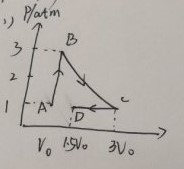
\includegraphics[width=0.35\textwidth]{Chp11_23.jpeg}
\end{figure}

(2)%gxf对原解答做了改动
\[\nu  = \frac{m}{M} = 0.1\mathrm{mol}\]
\[\frac{T_B}{T_A}=\frac{p_B}{V_B}{p_A}{V_A} = 3 \Rightarrow {T_B} = 3{T_A} = 900\mathrm{K}\]
同理,$\frac{T_D}{T_C}=0.5$,且有$T_C=T_B$,则:
\[\Delta E =\nu {C_V}({T_D}-{T_A})= 311\mathrm{J}\]
\[A =\nu R{T_B}\ln \frac{3{V_0}}{V_0}-\frac{{3P_0V_0}}{2}\]
由${p_0}{V_0} = nR{T_A}$得:
\[\frac{{3{p_0}{V_0}}}{2} = 374.13\mathrm{J}\]
则\[A = 450.65\mathrm{J}\]
\[Q = \Delta E+A = 762.42\mathrm{J}\]

\exercise

\solve 由下一章知识,\[{C_V} = \frac{i}{2}R,{C_p} = \frac{{i + 2}}{2}R\]
则
\[\gamma=\frac{{i + 2}}{i}\]
因为是绝热过程,则有
\[{T_0}{V_0}^{\gamma-1}={T_\text{\RNum{1}}}{(\frac{V_0}{2})^{\gamma-1}}= {T_\text{\RNum{2}}}{(\frac{{3{V_0}}}{2})^{\gamma-1}}\]
解得
\[{T_\text{\RNum{1}}} = {2^{\frac{2}{i}}}{T_0},{T_\text{\RNum{2}}} = {(\frac{2}{3})^{\frac{2}{i}}}{T_0}\]
则
\[A = \frac{{\nu R}}{{\gamma-1}}({(\frac{2}{3})^{\frac{2}{i}}}{T_0} - {T_0}) + \frac{{\nu R}}{{\gamma  - 1}}({2^{\frac{2}{i}}}{T_0}-{T_0}) = \frac{{i\nu R{T_0}}}{2}[{(\frac{2}{3})^{\frac{2}{i}}} + {2^{\frac{2}{i}}} - 2]\]
\chapter{气体动理论}
\section{选择题}
\exercise B

\solve 微观上,气体温度表示气体分子的运动速度,对于单个或少数分子,温度的概念失去了意义。宏观上,气体的温度表示气体分子的平均冷热程度。

\exercise B

\solve
\begin{gather*} 
{Vp=\sqrt{\frac{2kT}{u}}}\\
{u\left(\ce{O2}\right)}>u\left(\ce{H2}\right)\\
{Vp\left(\ce{O2}\right)<Vp\left(\ce{H2}\right) } \\
\frac{Vp\left(\ce{O2}\right)}{Vp\left(\ce{H2}\right)}=\sqrt{\frac{2kT}{32}} \sqrt{\frac{2kT}{2}}=\frac{1}{4}%需要长斜杠分数线
\end{gather*}
K为常量,T相同。

\exercise C

\solve 自由度为i的分子的平均动能为ikT/2。

\exercise A

\solve

$$
\begin{aligned} \sqrt {\bar{v^{2}}} &=\sqrt{\frac{3kT}{u}} \\
u\left(\ce{H2}\right)& > u\left(\ce{H2}\right) \\
\sqrt {\bar{v^{2}}\left(\ce{O2}\right)}& = \sqrt {\bar{v^{2}}\left(\ce{H2}\right) }\\
T\left(\ce{O2}\right)&>T\left(\ce{H2}\right) 
\end{aligned}
$$

\exercise B

\solve 等温过程系统内能不变。

\exercise A

\solve

\begin{gather*}
\varepsilon_{\ce{He}}=\varepsilon_{\ce{N2}}\\
n_{\ce{He}}=n_{\ce{N2}}\quad n=\frac{N}{V}\\
\bar{\varepsilon}=\frac{3}{2}kT\\
T_{\ce{He}}=T_{\ce{N2}}\\
p=\frac{2}{3}n\bar{\varepsilon}\\
p_{\ce{He}}=p_{\ce{N2}}
\end{gather*}

\exercise A

\solve

$$
\begin{aligned} 
p V & = \nu R T \\ p V & = \frac { m } { M } R T \\
p V & = \rho R T \\
\rho & = \frac { p M } { R T }
\end{aligned}
$$

由于水滴静止,则
$$
p_{\ce{H2}} =p_{\ce{O2}}
$$

又因为T相同,则

$$
\frac { p _ {\ce{H2}} } { p _ {\ce{O2}} } = \frac { \frac { p M _ {\ce{H2}} } { R T } } { \frac { p M_{\ce{O2}}}{ R T}}=\frac{1}{16}
$$

\exercise D

\solve

$$
\begin{aligned}
 \bar { z } & = \sqrt { 2 } \pi d ^ { 2 } \bar { v } n \\ \lambda & = \frac { 1 } { \sqrt { 2 } \pi d ^ { 2 } n } 
\end{aligned}
$$

$$
\because n = \frac { p } { k T }
$$不变,$ \bar { v }$不变

$$
\bar { z } = \sqrt { 2 } \pi d ^ { 2 } \bar { v } \frac { p } { k T },p
$$变为原来的两倍

$$
\begin{array} { l } 
{ \therefore z ^ { \prime } = 2 \bar { z } } \\ 
{ \because \bar { v } = \bar { \lambda } \bar { z } } \\
 { \therefore \lambda ^ { \prime } = 2 \bar { \lambda } }
\end{array}
$$

\exercise C

\solve

$$
\begin{array} { l } 
{ 2\ce{H2O} = 2\ce{H2}+\ce{O2}}\\
{ E = v\frac{i}{2}RT} 
\end{array}
$$

对于刚性分子,双原子分子气体的i=5,多原子分子气体的i=6

$$
\begin{array} { l }
 E _ { 0 } = 2 \cdot \frac { 6 } { 2 } R T \\ E _ { 0 } ^ { \prime } = 2 \cdot \frac { 5 } { 2 } R T + \frac { 5 } { 2 } R T = \frac { 15 } { 2 } R T \\ \therefore \frac { 15 } { 2 } R T \div 6 R T = 125 \% 
\end{array}
$$

\exercise B

\solve

$$
\begin{aligned} 
\sqrt { \bar { v } ^ { 2 } } & = \sqrt { \frac { 3 k T } { u } } \\ T _ { 2 } & = \frac { 3 } { 2 } T _ { 1 } \\ T _ { 2 } = \left( \frac { 3 } { 2 } \right) ^ { 2 } T _ { 1 } & = 280 \times \frac { 9 } { 4 } = 630 
\end{aligned}
$$
\section{填空题}
\exercise 
$\int _ { v _ { 2 } } ^ { v _ { 2 } } f ( v ) N d v$
\qquad
$\frac { \int _ { v _ { 1 } } ^ { v _ { 2 } } v f ( v ) d v } { \int _ { v _ { 1 } } ^ { v _ { 2 } } f ( v )\di{v}}$
\qquad
$N \cdot \frac { 1 } { 2 } m \int _{v_1}^{v_ 2} v^2f( v )\di{v}$

\solve
(1)

$$
\begin{aligned} \frac { d N } { N } & = f ( v ) d v \\ d N & = N f ( v ) d v \\ N ^ { \prime } = & \int _ { v_1 } ^ { v _ { 2 } } N f ( v ) d v \end{aligned}
$$

(2)
$$v_1 \sim v_2 \mbox{的平均速度}=\frac{\mbox{这个区间里每个分子速度之和}}{\mbox{这个区间里分子总数}}\\= \frac { \int _ { v _ { 1 } } ^ { v _ { 2 } } v d N } { \int _ { v _ { 1 } } ^ { v _ { 2 } } d N } = \frac { N \int _ { v _ { 1 } } ^ { v _ { 2 } } v f ( v ) d v } { N \int _ { v _ { 1 } } ^ { v _ { 2 } } f ( v ) d v } = \\frac { \int _ { v _ {1 } } ^ { v _ { 2 } } v f ( v ) d v } { \int _ { v _ { 1 } } ^ { v _ { 2 } } f ( v ) d v }$$

(3)
$$\mbox{总平动动能之和=每个分子平动动能之和}= \int _ { v _ { 1 } } ^ { v _ { 2 } } \frac { 1 } { 2 } m v ^ { 2 } d N \\ =  \frac { 1 } { 2 } m N \int _ { v _ { 1 } } ^ { v _ { 2 } } v ^ { 2 } f ( v ) d v 
$$


\exercise $\frac { N _ { A } } { N _ { A } + N _ { B } } f _ { A } ( v ) + \frac { N _ { B } } { N _ { A } + N _ { B } } f _ { B } ( v )$

\solve $\frac{N_A}{N_A+N_B}$指的是A在混合气体里占比,B同理。由概率论知识可知,对概率密度求加权平均即得结果。



\exercise
$
n _ { 0 } e ^ { - \frac { m g z } { k T } }
\qquad
z = - \frac { k T \ln ^ { \frac { p } { p_0 } } } { m g }
$

\solve 由玻尔兹曼分布律:

$$
\begin{aligned} n & = n _ { 0 } e ^ { - \frac { m g z } { k T } } \\ p & = p _ { 0 } e ^ { - \frac { m g z } { k T } } \\ z & = - \frac { k T \ln ^ { \frac { p } { p _ { 0 } } } } { m g } \end{aligned}
$$

\exercise 升高\qquad 升高

\solve (1)温度应上升。因为高速运动的氧气瓶中的分子是在杂乱无章运动的基础上附加上x方向定向运动速度。氧气瓶静止下来后,气体分子与氧气瓶发生碰撞,高速的x方向定向运动动能通过分子之间的频繁碰撞逐步平均分配到y、z方向的热运动动能上去,所以温度上升。

(2)$pV=\nu RT$,$T$增大,$V,\nu,R$都不变,所以$p$增大。

\exercise $\frac{3kT}{2}$\qquad 温度是大量分子热运动的集体表现,对单个或少数分子来说,温度的概念就失去了意义。

\exercise $7.82 \times 10 ^ { 7 } s ^ { - 1 } \qquad5 \times 10 ^ { - 5 } \mathrm { cm }$

\solve
由$\bar { \lambda } = \frac { k T } { \sqrt { 2 } \pi d^2p }$,$\bar { \lambda } $和$\bar { v } $成反比.

$p _0= 1 \times 10 ^ { 5 }\mathrm{Pa}$

$p _1= 1 \times 10 ^ { 4 }\mathrm{Pa}$

${ \therefore\ \overline{\lambda^{\prime} } = 10 \bar { \lambda } = 5 \times 10 ^ { - 5 }\mathrm{ cm }}$

${ z ^{\prime } = \frac { 1 } { 10 } \bar { z } = 7.82 \times 10 ^ { 7 }\mathrm{s^{-1}}}$

\exercise 1:4:16\qquad 1:2:4

\solve

$$
\begin{array}{*{20}{c}}
 \sqrt { \bar { v } ^ { 2 } } = 1.73 \sqrt { \frac { R T } { M } } \\ \because \sqrt { \bar { v } _ { A } ^ { 2 } } : \sqrt { \bar { v } _ { B } ^ { 2 } }  : \sqrt { \bar { v } _ { C } ^ { 2 } } = 1 : 2 : 4 \\ \therefore T _ { A } : T _ { B } : T _ { C } = 1 : 2 ^ { 2 } : 4 ^ { 2 } = 1 : 4 : 16 \\ n = \frac { N } { V } = \frac { \nu N _ { A } } { V } \\ \therefore n \propto \frac { \nu } { V }\\ \therefore \frac { \nu _ { 1 } } { V _ { 1 } } : \frac { \nu _ { 2 } } { V _ { 2 } } : \frac { \nu _ { 3 } } { V _ { 3 } }  = n _ { 1 } : n _ { 2 } : n _ { 3 } = 4 : 2 : 1 \\ p V  = \nu R T \\ p = \frac { \nu R T } { V }  = \frac { \nu } { V } \cdot T \cdot R \\ \therefore p  \propto \frac { \nu } { V } T \\ \therefore p _ { 1 } : p _ { 2 } : p _ { 3 } = 4 \times 1 : 2 \times 4 : 1 \times 16 = 1 : 2 : 4  
\end{array}
$$

\exercise 6

\solve (1)刚性多原子分子(甲烷)共有6个自由度。

(2)由于分子热运动的无规则性,任何一种运动都不比其他运动占有特别的优越性,所以机会相等,所以分子绕其质心转动对$i$的贡献为3.

\exercise $\geqslant 0 $\qquad 不变 \qquad 增

\solve
(1)孤立系统的熵永远也不会减少。

(2)可逆过程熵不变。

(3)由于ΔS$\geqslant 0$,不可逆过程熵增。


\exercise 0 \qquad 增

\solve(1)气体自由膨胀,对外界不做功(A=0)。绝热过程Q=0,ΔE=-A=0。故内能增量为0。

(2)孤立系统的熵永远也不会减少。


\section{计算题}
\exercise

\solve
(1)
\begin{figure}[!ht]
	\centering
	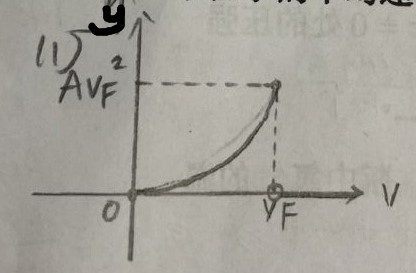
\includegraphics[width=0.35\textwidth]{./pics/Chp12_21.jpg}
\end{figure}

(2)
\begin{align*}
\int _ { 0 } ^ {+\infty}f(v)\di{v}
&=\int _ { 0 } ^ {v_F}Av^2\di{v}\\
&=\left. \dfrac { 1 } { 3 } A v ^ { 3 } \right| _ { 0 } ^ { v _ { F } }\\
&=\dfrac { 1 } { 3 } A v_F^3= 1 \\ 
A&=\dfrac{3}{ v_F^3 }
\end{align*}

(3)
速率分布曲线上与速率分布函数极大值所对应的速率称为最概然速率。

\therefore $v_P=v_F$

(4)
\begin{gather*}
{ \bar { v } = \int _ { 0 } ^ { v _ { F } } v f ( v ) d v } \\
 { \bar { v } = \int _ { 0 } ^ { v _ { F } } v \cdot \frac { 3 } { v _ { F } ^ { 3 } } v ^ { 2 } d v = \left. \frac { 3 } { 4 v _ { F } ^ { 3 } } v ^ { 4 } \right| _ { 0 } ^ { v _ { F } } = \frac { 3 } { 4 } v _ { F } } 
\end{gather*}

(5)
\begin{gather*}
 { \bar { v } = \int _ { 0 } ^ { v _ { F } } v f ( v ) d v } \\
{ \bar { v } = \int _ { 0 } ^ { v _ { F } } v \cdot \frac { 3 } { v _ { F } ^ { 3 } } v ^ { 2 } d v = \left. \frac { 3 } { 4 v _ { F } ^ { 3 } } v ^ { 4 } \right| _ { 0 } ^ { v _ { F } } = \frac { 3 } { 4 } v _ { F } } \\ { \bar { v } ^ { \prime } = \int _ { \frac { v _ { F } } { 2 } } ^ { v _ { F } } \frac { 3 } { v _ { F } ^ { 3 } } v ^ { 3 } d v = \left. \frac { 3 } { 4 v _ { F } ^ { 3 } } v ^ { 4 } \right| _ { \frac { v _ { F } } { 2 } } ^ { v _ { F } } = \frac { 3 } { 4 v _ { F } ^ { 3 } } \left( v _ { F } ^ { 4 } - \frac { 1 } { 16 } v _ { F } ^ { 4 } \right) = \frac { 45 } { 64 } v _ { F } }
\end{gather*}

\exercise

\solve
(1)
\begin{gather*}
{ p = n k T } \\ 
{ n = \frac { p } { k T } = 2.415 \times 10 ^ { 25 } } \\ 
{ n ^ { \prime } = 2.415 \times 10 ^ { 16 } } \\
 { \therefore N = 2.415 \times 10 ^ { 16 } \mbox{个} } 
\end{gather*}

(2)
$$
m _ { 0 } = \frac { M } { N _ { A } } = 5.31 \times 10 ^ { - 23 } g
$$

(3)
$$
\rho = \frac { m } { V } = \frac { N m _ { 0 } } { V } = \frac { 2.415 \times 10 ^ { 16 } \times 5.31 \times 10 ^ { - 23 } } { 10 ^ { - 9 } } \times 10 ^ { - 3 } = 1.28236 \times 10 ^ { 27 } \mathrm { kg } / \mathrm { m } ^ { 3 }
$$

(4)
$$
\bar { v } = \sqrt { \frac { 8 k T } { \pi m _ { 0 } } } = \sqrt { \frac { 8 \times 1.38 \times 10 ^ { - 23 } \times 300 } { \pi \times 5.31 \times 10 ^ { - 23 } \times 10 ^ { - 3 } } } = 446 \mathrm { m } / \mathrm { s }
$$

\exercise

\solve
(1)
$$
p = p _ { 0 } e ^ { - \frac { \mu g h } { k T } } = p _ { 0 } e ^ { - \frac { M g h } { R T } } = 0.633 p _ { 0 } = 6.45 \times 10 ^ { 4 } P a
$$
(2)
每口吸入的空气v不随海拔变化而变化。

相同质量$\rightarrow v $相同。

$pV=nRT$

忽略气温随高度变化时,T为定值。

$$
\begin{array}{l}
\therefore p_{0}\cdot 17 v =0.633p_0 \cdot x v\\
{ x = 26.7 \approx 27} 
\end{array}
$$
\exercise

\solve
(1)
$$
\begin{array} { c } { \rho = \frac { m } { V } = \frac { \nu m _ { 0 } } { V } = 11.3 g / c m ^ { 3 } } \\ { p V = \nu R T } \\ { \therefore \frac { \nu } { V } = \frac { p } { R T } = \frac { 1.01 \times 10 ^ { 3 } } { 8.314 \times 300 } = 0.405 } \\ { m _ { 0 } = \rho \frac { V } { \nu } = \frac { 11.3 } { 0.405 } = 27.9012 \approx 28 } \end{array}
$$

则可能是\ce{N2},\ce{CO},\ce{CH2=CH2}

(2)
$$
\sqrt{\bar{v^{2}}}=\sqrt {\frac{3kT}{\mu}}=1.73\sqrt {\frac{RT}{M}}=1.73\times\sqrt{\frac{8.314\times 300}{28\times10^{-3}}}=516.8\mathrm{m}/\mathrm{s}
$$

(3)
\begin{align*}
\bar{\varepsilon_{\mbox{平}}}&=\frac{3}{2}kT\\
&=\frac{3}{2}\times 1.38\times 10^{-23}\times 300\\
&=6.21\times 10^{-21}\\
\bar{\varepsilon_{\mbox{转}}}&=kT\\
&=4.14\times 10^{-21}
\end{align*}

(4)单位体积总平动动能=1个分子平均平动动能*分子数密度

$$E_{\mbox{平总}}=\bar { \varepsilon } _ {\mbox{平}}n=\bar { \varepsilon } _ {\mbox{平}}\frac{p}{kT}=6.21 \times 10 ^ { - 21 } \times \frac { 1.01 \times 10 ^ { 3 } } { 1.38 \times 10 ^ { - 23 } \times 300 } = 1515 J$$

同理,$\bar { \varepsilon } _ {\mbox{转总}}=1010J$

(5)
$$
E = \nu \frac { i } { 2 } R T = 0.3 \times \frac { 5 } { 2 } \times 8.314 \times 300 = 1870.65 J
$$
\chapter{机械振动}
\section{选择题}
\exercise A

\solve
由图可知,简谐振动的周期介于2至4之间,因此角频率介于0.5$\pi$和$\pi$之间,排除C,D。又由于带入t=2,应有$x=A=2$,故仅有A选项满足要求。

\exercise B

\solve
设弹簧振子的振动方程为$x=A\cos(\omega t+\varphi_0)$,则速度方程为$v=\frac{dx}{dt}=A\omega\cos(\omega t+\varphi_0+\frac{\pi}{2})$,故振幅增大一倍,速度亦增大一倍,选B。

\exercise C

\solve
动能与振子速度的平方成正比,且在振子速度最大时,动能等于振动总能量。因此,此时动能与动能总能量的比等于$\cos^2(\omega t+\varphi_0+\frac{\pi}{2})$。又由于此时位移大小为振幅的$\frac{1}{4}$,知$\cos(\omega t+\varphi_0)=\frac{1}{4}$,故$\cos^2(\omega t+\varphi_0+\frac{\pi}{2})=1-\cos^2(\omega t+\varphi_0)=1-\left(\frac{1}{4}\right)^2=\frac{15}{16}$,选C。

\exercise C

\solve
由图可知,$v|_{t=0}=\frac{1}{2}v_{max}$,又由于图像为余弦函数右移后图像,知速度初相位为$-\frac{\pi}{3}$。若设位移初相位为$\varphi_0$,则速度初相位为$\varphi_0+\frac{\pi}{2}=-\frac{\pi}{3}$,因此$\varphi_0=-5\frac{\pi}{6}$,选D。

\exercise A

\solve
机械振动的角速度$\omega=\sqrt{\frac{a_{max}}{x_{max}}}=\sqrt{\frac{a_m}{A}}$,因此周期$T=\frac{2\pi}{\omega}=2\pi\sqrt{A/a_m}$,A选项正确,B选项错误。\par
通过平衡位置的总能量等于动能$E=\frac{1}{2}mv{_{max}}^2=\frac{1}{2}ma{_m}A$,故CD错误,选A。

\exercise A

\solve
由于起点时刻位移为$\frac{1}{2}A$,A、B选项符合要求。又由于起始时刻向x轴负方向运动,仅有A选项满足要求。

\exercise E

\solve
动能方程只能表示速度的大小,而不能表示初始状态下速度方向,因此最后一定有两个相差$\pi$的可能初始相位,因此选E。

\exercise A

\solve
弹簧振子的劲度系数与长度反比,因此每根短弹簧的劲度系数为3k。并联以后,物体受力为三根弹簧受力之和,因此相当于一根劲度系数为9k的弹簧。因此弹簧振子的周期$T=2\pi\sqrt{\frac{m}{k'}}=\frac{2\pi}{3}\sqrt{\frac{m}{k}}$,选A。

\exercise B

\solve 
由题可知,第二个质点的加速度到达正向最大(对应位移负向最大)时,第一个质点在平衡位置向正向移动。因此第二个点比第一个落后1/4个周期,也即$\pi/2$个相位。因此选B。

\exercise B

\solve
拍频等于两个音叉固有频率的差的绝对值,因此A、B选项满足要求。又由于周期$T=2\pi\sqrt{\frac{k}{m}}$,因此挂上重物后,待测音叉的震动周期变长,频率减小。由于此时的拍频也减小,说明待测音叉的固有频率是高于标准音叉的,选B。

\section{填空题}
\exercise 不是

\solve 
见教材75页,同方向不同频率谐运动的合成后振幅随时间变化,不是简谐运动。

\exercise $0.5\mathrm{cm}$ \quad $x=0.5cos(\pi t+\pi)$

\solve
初始状态速度为0,因此处在位移负向最大状态,故振幅为0.5cm,初相位为$\pi$。又由于频率为0.5Hz,知角频率为$\pi$Hz,即振动方程为$x=0.5cos(\pi t+\pi)$
 
\exercise $\frac{\sqrt{7}}{2}$ \quad $\arctan{\frac{2\sqrt{3}}{3}}$

\solve
\begin{figure}[htbp]
\centering
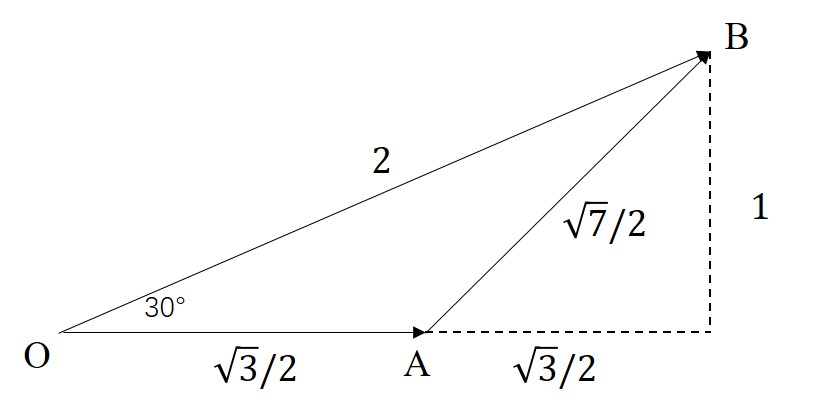
\includegraphics[height=4.7cm,width=9.5cm]{./pics/Chp13_13.jpg}
\caption{简谐运动矢量叠加图}
\end{figure}
如图绘制出简谐运动的矢量叠加图,其中OA,AB分别为第一,第二个简谐振动,OB为叠加后的简谐振动。在已知OA、AB大小方向的前提下,由几何关系即可以计算出OB的大小(即第二个简谐振动的振幅)以及两个简谐振动的相位差。

\exercise $\frac{T}{24} \quad \frac{7T}{24}$

\solve
由于速度始终比位移提前1/4个周期,而动能,势能分别与速度的平方、位移的平方成正比,因此当且仅当相位为$\pm\frac{\pi}{4}$或$\pm\frac{3\pi}{4}$ 时,动能与势能相等。因此,在半个周期内,两个动能与势能相等的时刻分别为$t_1=\frac{T}{2\pi}\left(\frac{\pi}{4}-\frac{\pi}{6}\right)=\frac{T}{24}, t_2=\frac{T}{2\pi}\left(\frac{3\pi}{4}-\frac{\pi}{6}\right)=\frac{7T}{24}$。

\exercise $0.03\cos(\frac{\pi}{2}t-\frac{\pi}{2})$

\solve
由图可知,两个简谐运动的振动方程分别为$x_1=0.06\cos(\frac{\pi}{2}t-\frac{\pi}{2})$,$x_2=-0.03\cos(\frac{\pi}{2}t-\frac{\pi}{2})$,相加后即可算出合振动的方程为$x=0.03\cos(\frac{\pi}{2}t-\frac{\pi}{2})$。

\exercise $3$

\solve
由图可知,图像为向右平移了$\frac{\pi}{3}$的余弦曲线,因此初始时刻的相位为$-\frac{\pi}{3}$,另一个x为1的点的相位与初始点关于相位为$\frac{\pi}{2}$对称,因此经过$\frac{2\pi}{3}$的角位移所需的时间为1s,由于一个周期对应$2\pi$的角位移,因此振动的周期为3s。

\exercise $\frac{3}{4}E \quad \frac{1}{4}E \quad \pm\frac{\sqrt{2}}{2}A$

\solve
弹簧振子的弹性势能与位移的平方成正比,因此当位移是振幅的一半时,弹性势能是最大弹性势能的1/4。注意到最大弹性势能与总能量$E$相等,故势能$E_p=\frac{1}{4}E$,动能$E_k=E-E_p=\frac{3}{4}E$。同理,当动能与势能相等,均为总能量一半时,位移的大小应为振幅的$\frac{\sqrt{2}}{2}$倍,即位移为$\pm\frac{\sqrt{2}}{2}A$。

\exercise $0.05\mathrm{m}\quad -\arccos{\frac{3}{5}}$

\solve
对$x$求导有$v=3A\cos(3t+\varphi+\frac{\pi}{2})$,故由题意知,$x(0)=A\cos\varphi=0.03,v(0)=3A\cos(\varphi+\frac{\pi}{2})=0.12$,联立两式即可解出$A$与$\varphi$的值。

\exercise $\sqrt{2}:\sqrt{3}$

\solve
单摆的周期$T=2\pi\sqrt{\frac{l}{g}}$,因此周期正比于绳长的平方根。由于左右两边的绳长比为2:3,周期比为$\sqrt{2}:\sqrt{3}$。

\exercise

\solve
\begin{figure}[htb]
\centering
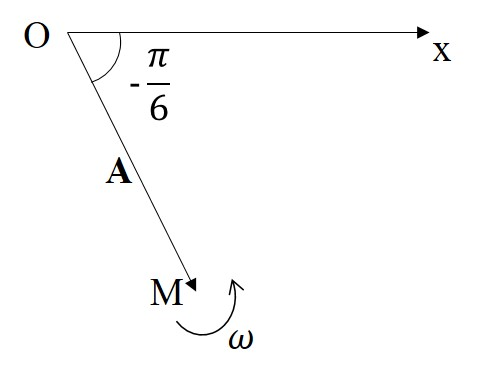
\includegraphics[height=3.7cm,width=5cm]{./pics/Chp13_20.jpg}
\caption{旋转矢量图}
\end{figure}
具体绘图方法见教材72页。

\section{计算题}
\exercise

\solve
(1)加速度$a=\frac{F}{m}=-2x$,因此角频率$\omega=\sqrt{\frac{a}{-x}}=\sqrt{2}$,故周期为$T=\frac{2\pi}{\omega}=\sqrt{2}\pi$。

(2)由于动能的最大值等于势能的最大值,有:$E_{\text{动}max}=E_{\text{势}max}=\frac{1}{2}kA^2=0.0675$J

\exercise

\solve
(1)振动的角频率$\omega=\frac{2\pi}{T}=\pi$Hz。撤去外力后,物体处于正向位移最大,负向加速度最大的状态,而撤去外力前,物体平衡。因此,撤去的外力大小等于物体振动过程中的受力最大值,即$F=ma_{max}=mA\omega^2=0.493$N

(2)弹簧的弹性系数$k=F/A=4.93$N/m,因此振动系统的总能量(与弹性势能最大值相等)为$E_{max}=\frac{1}{2}kx^2=0.0247$J。由于势能与相对平衡位置的位移的平方正比,当物体在平衡位置以下5cm,即最大位移的1/2处时,势能是最大势能(也就是总能量)的1/4,因此$E_p=\frac{1}{4}E_{max}=0.00617$J,而动能$E_ k=E_{max}-E_ p=0.0185$J

\exercise

\solve
设单摆振动方程为$x=A\cos(\omega t+\varphi_0)$,则速度方程为$v=\frac{dx}{dt}=A\omega\cos(\omega t+\varphi_0+\frac{\pi}{2})$。故由题意知,
\begin{equation*}
  \left\{
   \begin{array}{c}
   x(0)=A\cos{\varphi_0} = -5  \\
   v(0)=A\omega\cos(\varphi_0+\frac{\pi}{2}) = -10  \\
   \omega=\sqrt{\frac{g}{l}}=2.89{\rm Hz}   \\
   \end{array}
  \right.
\end{equation*}
解方程得,振幅$A=6.08$cm,初相${\varphi_0}=1.57$rad\\
另一方面,周期$T=\frac{2\pi}{\omega}=2.18$s

\exercise

\solve
以向右为正方向,设A的加速度为$a$,相对弹簧自由状态的位置为$x$。首先对A水平受力分析,A受到弹簧的力$F_1=-kx$,以及AB间绳的拉力$F_2$。为求出$F_2$,再对滑轮受力分析。滑轮转动惯量$J=\frac{mR^2}{2}$,角加速度$\beta=a/R$,右端拉力为$m_2g$,因此左端拉力$F_2=m_2g-\frac{J\beta}{R}=m_2(g-a)-0.5ma$
故A的合力$F=F1+F2=-kx+m_2(g-a)-0.5ma$,于是可以推导出a的加速度方程:
\begin{equation*}
\begin{split}
a=\frac{-kx-0.5ma+m_2(g-a)}{m_1}\\
a=\frac{-kx-0.5ma+m_2g}{m_1+m_2}\\
(1+\frac{m}{2m_1+2m_2})a=-\frac{k}{m_1+m_2}x+\frac{m_2}{m_1+m_2}g\\
a=-\frac{2k}{2m_1+2m_2+m}(x+x_0)
\end{split}
\end{equation*}
其中,$x_0=\frac{2m_2g}{2k}$。于是,角频率$\omega=\sqrt{\frac{a}{-x}}=\sqrt{\frac{2k}{2m_1+2m_2+m}}$

\chapter{机械波}

\section{选择题}

\exercise C

\solve 由波动方程的式子$y=0.08cos(10\pi t-4\pi x)$(SI)

知圆频率$\omega=10\pi$,频率$f=\frac{\omega}{2 \pi}=5Hz$;

知$2\pi\lambda=4\pi$,得波长$\lambda=0.5m$,得波速$u=\lambda f=2.5m/s$。

根据以上结果排除选项,知答案为D。

\exercise D

\solve 

选项A:$x$前系数为负,说明波正向传播,错误;

选项B:将方程化为标准形式:$y=Acos(a(bt-x)-\phi)$,可以看出$x$前系数为负,说明波正向传播,错误;

选项C:由波动方程知,在$x$轴上有些点永远不会振动(是驻波方程),不是行波,错误;

选项D:方程有$y=Acos(ax+t)+Acos(ax+t-\phi)$,则每一个位置的振动都可以看成是两个等振幅等圆频率的振动的合成,一定可以合成为$y=Acos(ax+t+\phi_2)$的形式;而合成振动的$x$前的系数为正,则是负向传播,正确。

\exercise A

\solve 将$t=0.5s$带入$y=0.20cos[2\pi (t-x/2)+\pi]$得$y(x,0.5)=0.20cos(\pi x)$,由图像可知选A。

\exercise D

\solve 由图像的最高点可知振幅$A=\sqrt{2}m$,由周期$T=4s$,波长$\lambda=4m$,及波沿x轴正向传播,得波函数为$y=\sqrt{2}cos[2\pi({\frac{t}{T}-\frac{x}{\lambda}})+\phi_0]=\sqrt{2}cos(\frac{\pi}{2}(t-x)+\phi_0)$。则$y(0,t)=\sqrt{2}cos(\frac{\pi}{2}t+\phi_0)$,由图中可知$\sqrt{2}cos\phi_0=-\frac{\sqrt{2}}{2}$,又由此时$x=0$处质点在$t=0$处即将向下运动知,$\phi_0=\frac{2}{3}\pi$。则有$y=\sqrt{2}cos(\frac{\pi}{2}(t-x)+\frac{2}{3}\pi)$,选D。

\exercise C

\solve  由图中可得振幅$A=0.01$m,波长$\lambda=200$m,频率$f=\frac{u}{\lambda}=1$Hz,周期$T=\frac{1}{f}=1\mathrm{s}$。由于周期为$1\mathrm{s}$,则$t=1\mathrm{s}$和$t=0\mathrm{s}$的振动情况是一样的。设P的振动方程为$y=0.01cos(2\pi\frac{t}{T}+\phi_0)=0.01cos(2\pi t+\phi_0)$。而在$t=0\mathrm{s}$时,有$cos(\phi_0)=0.5$,且P点将向下运动,则$\phi_0=\frac{1}{3}\pi$。

综上所述,P点的运动方程为$y=0.01cos(2\pi t+\frac{1}{3}\pi)$,选C。

\exercise D

\solve  设在$r$处,波的单位面积能量为$B=kI$,则以波源为中心,以$r$为半径上的球面的总能量为$E=4\pi r^2 kI$。而由能量守恒知,不同球面上波的总能量是相同的,所以有$E=C$(常量),则$I=\frac{C}{4\pi k r^2}$。则有$I\propto \frac{1}{r^2}$,选D。

\exercise D

\solve 由图中位置关系可知,$S_1$到达P点比$S_2$到达P点超前$\frac{\lambda}{2}$。则$S_1$和$S_2$的相位差为$\phi_1-\phi_2=\frac{ 2\pi\lambda}{2 \lambda}+\frac{\pi}{2}=\frac{3\pi}{2}$,选D。 

\exercise A

\solve 两列波到达P点的相位差为$\Delta\phi=\frac{2\pi\Delta x}{\lambda}=\frac{2\pi\Delta x f}{u}$。

由于在P点相消干涉,则$\Delta\phi=(2k+1)\pi$。

有$f=\frac{u}{2\Delta x}(2k+1)=\frac{172}{1.3}(2k+1)$。

为使$1350\leqslant f \leqslant 1826$,取k=6,有$f=1720Hz$,选A。

\exercise D

\solve 弦上产生的驻波的频率要满足$u=\frac{u}{2f}k,k=1,2\ldots$。则不能产生任意频率,排除AB。

在微小横振动时,质元的势能$E_p\propto (\frac{\partial y}{\partial x}|_x)^2$,即质元所在位置的弦的斜率的平方越大,此处势能越大。则在弦上各点达到最大位移时,在波节处的质元斜率平方最大,则在波节处质元的势能最大,选D。

\exercise D

\solve 由多普勒效应,在波源与观察者相向而行时,有$f=\frac{u+v_1}{u-v_2}f_0$,其中$v_1$是观察者即火车的速度,$v_2$是波源即汽车的速度,$u$是空气中声速。计算得$f=1.2548kHz$,最接近为D选项,选D。

\section{填空题}
\exercise $1.2\mathrm{m}$\qquad$0.1\mathrm{m}$

\solve 波长$\lambda=uT=1.2\mathrm{m}$;

由于两点在波的传播方向上,则相位差有$\Delta \phi=\frac{2\pi \Delta x}{\lambda}$,则计算得$\Delta x=0.1\mathrm{m}$。

\exercise $\frac{2\pi}{k}\qquad Acos(\omega t+\pi)\qquad -\frac{1}{2}\frac{\rho \omega^3}{k}A^2$

\solve 由于机械波向$x$轴负向传播,则有$k=\frac{2\pi}{\lambda}$,得到$\lambda=\frac{2\pi}{k}$;

将$x=\frac{\lambda}{2}=\frac{\pi}{k}$代入,得$y(\frac{\pi}{k},t)=Acos(\omega t+k\frac{\pi}{k})=Acos(\omega t+\pi)$;

平均能流密度为$\textbf{I}=\bar{w}\textbf{u}$。而波的平均能量密度为$\bar{w}=\frac{1}{2}\rho A^2 \omega^2$,又知波沿x轴负方向传播,故$u=-\frac{\omega}{k}$。则$I=-\frac{1}{2}\frac{\rho \omega^3}{k}A^2$。

\exercise 0.6$\qquad$30

\solve 相位差与间距有关系$\Delta \phi=\frac{2\pi \Delta x}{\lambda}$,则有$\lambda=\frac{2\pi \Delta x}{\Delta \phi}=0.6\mathrm{m}$,波速$u=\lambda f=30\mathrm{m/s}$。

\exercise 减小

\solve 由于A处质元的弹性势能在减小,则此时A向上运动,则A的速度减小,则振动动能减小。

\exercise $40\qquad D,E \qquad -20$

\solve 此时A点为两个波峰叠加,高度为20cm,B点为两个波谷叠加,高度为-20cm,则A,B两点的高度差为40cm,且A,B两点均为振动加强的点;

由于D,E点在此时均由波峰和波谷相遇合成,故D,E点为振动减弱点,而C点在A,B所连线段中间,故也是振动加强点;

由于C点是振动加强点,则C点的振幅为20cm,在此时刻C点高度为0,且下一时刻向下运动,故此时C点的相位为$\frac{\pi}{2}$;由$\omega=\frac{2\pi u}{\lambda}=10\pi\ \mathrm{rad/s}$,得经过$\Delta t=0.65\mathrm{s}$后,相位增加$\Delta \phi=\omega\Delta t=6.5\pi$,则C点的振动相位为$\phi=0.5\pi+6.5\pi=7\pi$,C点为波谷,故高度(位移)为-20cm。

\exercise 不同$\qquad$相同

\solve 驻波方程为$y=Acos(\frac{2\pi x}{\lambda})cos(\frac{2\pi t}{T}+\phi_0)$,则在相邻波节之间,各点的振幅为$|Acos(\frac{2\pi x}{\lambda})|$,振幅不相同;同时相邻波节之间$Acos(\frac{2\pi x}{\lambda})$总是同正负,则相位总是相同。

\exercise \pi

\solve 由驻波方程可知,在$x_1$处的振动为$y_1=\frac{\sqrt{2}}{2}Acos(15\pi t)$,在$x_2$处的振动为$y_2=-\frac{\sqrt{2}}{2}Acos(15\pi t)=\frac{\sqrt{2}}{2}Acos(15\pi t+\pi)$。则两个振动的相位相差\pi。

\exercise 光疏介质$\qquad$光密介质

\solve 根据定义,一列光波从一种介质向另一种介质入射,光速较大的介质叫做光疏介质,光速较小的叫做光密介质。

\exercise 朝向$\qquad$0.25

\solve 设空气中声速为$u_0$,设声源朝向观察者的速度是$u$。则观察者接收到的波长$\lambda=\frac{u_0-u}{u_0}\lambda_0=\frac{3\lambda_0}{4}$,解出$u=\frac{1}{4}u_0=0.25u_0$。由于解出u大于0,则声源朝向观察者运动,且运动速度为空气中声速的0.25倍。

\exercise 8.48m/s

\solve 设潜艇移动的速度为$u$,则在潜艇接收到的信号频率为$f_1=\frac{u_0+u}{u_0}f_0$,则潜艇反射的信号频率为$f=\frac{u_0}{u_0-u}f_1=\frac{u_0+u}{u_0-u}f_0$。可知探测器接收到的信号频率增大,则$f-f_0=341$,得$f=30341Hz$。已知$u_0=1500\mathrm{m/s}$,代入计算得$u=8.48\mathrm{m/s}$。


\section{计算题}
\exercise

\solve (1)由于波向x正向传播,则在$x$处的质点,振动的相位比$0.1$m处的质点落后$\Delta \phi(x)=\frac{\omega}{u}(x-0.1)$。而在0.1m处的质点振动为$y_0=0.5sin(1.0-4.0t)=0.5cos(4t-1+\frac{\pi}{2})$。则可得圆频率$\omega=4\mathrm{rad/s}$,则$\Delta \phi(x)=5(x-0.1)$。

由以上可得$y(x,t)=0.5cos(4t-1+0.5\pi-5(x-0.1))=0.5cos(4t-5x+1.07)\mathrm{m}$

(2)$v(0.1,t)=\dy{y(0.1,t)}{t}=-2sin(4t+0.57)\mathrm{m/s}$

(3)$v_{max}=2\mathrm{m/s}$;则$\frac{v_{max}}{u}=5:2=2.5$。

\exercise 

\solve 由坐标变换,有
\[
\begin{cases}
	x'=-(x-\frac{\lambda}{4})\\
	y'=y
\end{cases}
\]
即
\[
\begin{cases}
	x=\frac{\lambda}{4}-x'\\
	y=y'
\end{cases}
\]

将上式代入波动方程$y=Acos(2\pi(\frac{t}{T}-\frac{x}{\lambda})+\varphi)$,得新坐标下的波动方程为:

$$y'=Acos(2\pi(\frac{t}{T}+\frac{x'}{\lambda})+\varphi-\frac{\pi}{2})$$

\exercise

\solve (1)$f=\frac{1}{T}=2Hz$,$u=\lambda f=1.6\mathrm{m/s}$;(或$u=\frac{\lambda}{T}=1.6\mathrm{m/s}$)

(2)$y(x,t)=0.2cos(2\pi(\frac{t}{0.5}-\frac{x}{0.8})+\varphi_0)\mathrm{m}$;

而$y(0.2,t)=0.2cos(-\frac{\pi}{2}+\varphi_0)$,由$t=0$时,$x=0.2m$的质点处于反向最大位移处,则有$-\frac{\pi}{2}+\varphi_0=\pi$,则$\varphi_0=\frac{3\pi}{2}$。

则$y(x,t)=0.2cos(2\pi(\frac{t}{0.5}-\frac{x}{0.8})+\frac{3\pi}{2})\mathrm{m}$;

(3)$y(\frac{3}{4}\lambda,t)=0.2cos(4\pi t)\mathrm{m}$;

(4)$\Delta x=0.3\mathrm{m}$,$\Delta \varphi=\frac{\Delta x}{\lambda}2\pi=0.75\pi$。

\exercise

\solve (1)$y_1=Acos(2\pi(\frac{t}{T}-\frac{x}{\lambda})+\frac{3\pi}{2})\mathrm{m}$;

(2)反射波方向与入射波相反,但是振幅,频率和波速不变,故设反射波方程为$y_2=Acos(2\pi(\frac{t}{T}+\frac{x}{\lambda})+\frac{3\pi}{2}-\Delta \varphi)\mathrm{m}$。

而反射波到达原点时,相位比入射波落后$\Delta \varphi =2\times\frac{3}{4}\lambda\times \frac{2\pi}{\lambda}+\pi=4\pi$(其中最后加的$\pi$是半波损失的相位)。而$4\pi$是$2\pi$的整数倍,故不影响方程的形式。则有$y_2=Acos(2\pi(\frac{t}{T}+\frac{x}{\lambda})+\frac{3\pi}{2})\mathrm{m}$;

(3)$y=y_1+y_2=2Acos(\frac{2\pi x}{\lambda})cos(\frac{2\pi t}{T}+\frac{3\pi}{2})\mathrm{m}$

则当$cos(\frac{2\pi x}{\lambda})=0$时为波节,则$\frac{2\pi x}{\lambda}=\frac{2n+1}{2}\pi$,得$x=\frac{2n+1}{4}\lambda$,其中$n$是整数。则在图中$x=\frac{1}{4}\lambda,\frac{3}{4}\lambda$处标注为静止点。
\chapter{波动光学1(干涉)}
\section{选择题}
\exercise A

\solve 相干长度(书上P129):一切实际光源发射的光是一个个的波列,当两个分光束的光程差大于波列长度L时,将不能发生干涉现象。这个波列长度L成为该光源的相干长度。 

\exercise C

\solve 两束光不能观察到相干现象的本质是两束光不是相干光。相干光要求:频率相同,光矢量振动方向平行且具有恒定的相位差。

\exercise A

\solve 光源的空间相干性指的是光源的相干长度,由光源的线度决定。可以理解为光源本身的尺寸影响了光源发出的光的波列的长度。

\exercise C

\solve 由于一个狭缝的宽度变窄,说明其中一束光的光强变弱,但是其振动的频率和相位没有发生变化,故两束光仍然是相干光,仍然会发生干涉现象。由双缝干涉间距公式(公式三),可知条纹的间距不变。由于此时两束光的最大光强不同,故原来光强为零的地方现在不再为零。

\exercise A

\solve 振幅相等说明光强相等,则由此产生的光的干涉现象中,最小光强为零,最大光强为单束光光强的两倍。

\exercise A

\solve 本题考查介质中光程差的计算方法。由于加入玻璃片后,光在玻璃片中的光程差发生改变,增加了(n-1)d,即增加了5λ的光程差,故不影响原有的明纹暗纹分布,中央明纹处依旧是明纹。

\exercise D

\solve 解析:由于要研究透射光的相干现象。做出光路图(光路图一),由图可知两束光的光程差为2nd,由相长干涉的条件(公式四)可知最小厚度即为λ/(2n)。

\exercise B

\solve 解析:研究光的干涉现象的关键是要分析清楚光程差的变化情况。设凸透镜离开平玻璃的距离为l,由牛顿环的中心光程差(公式五),可知现在中心点的光程差为(公式六),随着l的增加光程差也在增加,故中心点的光程差将依次满足明纹暗纹的条件,故中心点会出现明纹暗纹交替的现象。对于第k级暗纹,原来的rk为(公式七),现在为(公式八),可知(公式九),故条纹向中心收缩。

\exercise C

\solve 注意审题,是从下向上观察,即观察透射光的干涉现象(类比第七题)。由于半波损失发生在光从光疏介质射向光密介质,在界面上发生反射时,由于玻璃的折射率为1.5,故两束光都没有半波损失,由出现暗纹的条件(公式十)可知最小距离为78.1nm。

\exercise B

\solve 扩展光源发出的波矢量方向极多,相干性很差,如白炽灯。但是同一个角度发出的光在屏幕上在同一个圆周上,可类比点电荷的电场线分布考虑。
\section{填空题}
\exercise $5\times10^{-7}\mathrm{m}$ 

\solve 由于光的相位的该变量为3π,那么光程差即为1.5λ,由频率可以求出波长,就可以求出介质薄片的厚度,具体如图:(图一)

\exercise 563.6

\solve 本题考查迈克尔逊干涉仪中的条纹距离公式,即δd=Nλ/2,代入相关数据即可解得。

\exercise $3d$

\solve  又是透射光的光程差问题,与第七题和第九题一样,此处不再赘述。

\exercise 两个次波源 \quad 相干波源 

\solve 书上介绍了两种获得相干光源的办法:分波阵面法和分振幅法。前者是在光源发出的同一波列的波面上取出两个次波源作为相干波源,如杨氏干涉。后者是把同一波列的波分为两束光波,如薄膜干涉。

\exercise 9λ/4n2

\solve (2是n的下角标) 做出光路图如图所示,由于两束光均为从光疏介质射向光密介质并且在界面分界出发生反射,故两束光均存在半波损失,故光程差没有半波损失。由干涉出现暗纹的条件可知厚度。(光路图二)

\exercise $(r1/r2)^2$

\solve 分别写出r1和r2的表达式,则可知液体的折射率。(公式十一)

\exercise $4*10^-5$

\solve 由劈尖干涉的公式(公式十二)可知sinθ的值,根据几何关系和小角度近似(公式十三)可知小纸条的厚度。

\exercise $xd/5D$

\solve 直接由杨氏双缝干涉中相邻的明纹或者暗纹之间的距离公式(公式十四),且第零级明纹和第五级明纹之间的距离为五个δx,故可知(公式十五)

\exercise 

\solve 对于一般位置分析,做出光路图(光路图三)可知光程差的表达式为(公式十六),在中心处由于d=0,故中心处的光程差为(公式十七),满足干涉出现暗纹的条件。

\exercise 

\solve 考查迈克尔逊干涉仪的相关概念。当M1撇和M2平行时,可观察到同心圆的条纹分布,这是等倾干涉。当M1撇和M2不平行时,由于空气隙的存在,会观察到类似于等厚干涉的等距直线条纹。

\section{解答题}

三.计算题
21. 本题考查劈尖干涉,只要能正确理解公式的含义就可以顺利解出,难度不大。
(图)

22.本题考查劈尖干涉的光程差的分析,由于条纹整体左移,说明光程差变大了,即左边的空气隙的厚度变大了,说明工件表面有凹陷,且可以定量算出凹陷的深度。
(图)

23.本题考查薄膜干涉的两种情况。如果观察反射光可以直接利用薄膜干涉的公式(公式十八),根据k的取值判断光的颜色。如果观察透射光,可以利用作业第七题,第九题提到的算法同样判断k的值得到光的颜色。
(图)

24.本题要求类比牛顿环的分析方法分析干涉现象,关键是要抓住光程差的分析,前两问非常基础。第三问关于疏密的判断可以类比第八题,即判断δr,由于δr是关于θ的单元函数,故可以由θ的变化判断出疏密的变化。
(图)


\chapter{波动光学2(衍射)}
\section{选择题}
\exercise A

\solve
由于形成中央亮条纹的光是垂直通过单缝,在经过聚透镜后会聚焦到光轴上。所以聚透镜向y轴正方向平移,则中央衍射条纹会向上移动。又因为中央亮条纹宽度为$k=1$与$k=-1$两条暗条纹之间的距离。则有$bsin\varphi=\pm2k\frac{\lambda}{2},k=1$,当$b$减小,则$\varphi$增大,又因为$tan\varphi=\frac{x_1}{f}$,所以$x_1$增大,即中央亮条纹会变宽。

\exercise B

\solve
要让分辨本领大,则最小分辨角$\delta_\varphi$要尽量小,又因为$\delta_\varphi=\varphi_0\approx1.22\frac{\lambda}{D}$,电子波长比可见光波长小,即$\lambda$小,则电子波的$\delta_\varphi$更小,分辨率更高。

\exercise D

\solve
\begin{figure}[htbp]
\centering
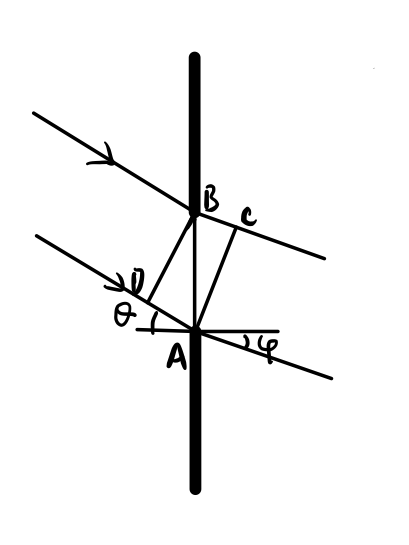
\includegraphics[width=0.25\linewidth]{Chp16_3.PNG}
\caption{1.3图}
\end{figure}
光程差$\Delta=BC-DA=a(sin\phi-sin\theta)$;

中央亮条纹满足$a(sin\phi-sin\theta)=0$,即$\phi=\theta$;

所以中央亮条纹会偏移$\theta$,所以移动的距离x=$ftan\theta$。

\exercise D

\solve
在进行光学测量时,条纹越亮、越细、分得越开,测量越精确。光栅衍射具有这样的效果。

\exercise C

\solve
由光栅方程$(a+b)sin\varphi=\pm k\lambda$。由于衍射光线的原因,即$asin\varphi=\pm k'\lambda$,$k'=1,2,3...$时出现暗条纹,即$k=k'\frac{a+b}{a}$=2k'时,原应该有的亮条纹会由于衍射变为暗条纹。除了中央亮条纹外,一边会出现3条亮条纹,其中$k=1,2,3...,k'=1,2,3...$即$k=2$时会出现暗条纹,即$k=1$时出现第一条明纹,$k=3$时出现第二条明纹。所以选C。

\exercise C

\solve
惠更斯-菲涅尔原理指的是从同一波前上各点发出的次波是相干波,经过传播在空间某点相遇时叠加是相干叠加。这条定理也适用光的干涉。

\exercise D

\solve
由最小分辨角公式$\delta_\varphi=\varphi_0\approx1.22\frac{\lambda}{D}$,带入数值算得$\delta_\varphi=5.3\times10^{-7}rad$。

\exercise

\solve B
对于中央亮条纹,它是由各色光同时合成的,所以为白色。又由于由紫光到红光的波长逐渐增大,又$asin\varphi=\pm k\lambda$,对于同级亮纹,波长越大,衍射方向角($\varphi$)越大。又由于几何关系得衍射方向角越大,在屏幕上的亮条纹离中央亮条纹越远。

\exercise B

\solve
由最小分辨角公式$\varphi_0\approx1.22\frac{\lambda}{D}$得,$\varphi=2.33\times10^{-4}rad$,所以物品大小为$l=\varphi\cdot H=2.33\times10^{-4}\times300\times10^{3}m=67.1m$。

\exercise C

\solve
由衍射公式$asin\varphi=\pm k\lambda$,以及几何关系$sin\varphi\approx tan\varphi=\frac{x}{f}$,解得宽度d=$2x=\frac{2\lambda f}{a}$,所以焦距f增大,d也增大。

\section{填空题}
\exercise 中心

\solve
由于规定最小分辨角通常采取瑞利判据,即一个圆斑像中心刚好落在另一圆斑像的第一级暗环上。

\exercise $2\lambda$

\solve
根据单缝衍射条纹的暗纹条件,即$asin\varphi=\pm2k\frac{\lambda}{2}$,在第二个暗条纹时,$k=2$。所以光程差$asin\varphi=2\lambda$。

\exercise $6.04\times10^{-5}\mathrm{m}$

\solve
根据单缝衍射条纹的暗纹条件,即$asin\varphi=\pm2k\frac{\lambda}{2}$,对于第一级暗条纹,$k=1$。其中$\varphi=1.2°/2=0.6°$,代入方程得$a=\frac{\lambda}{sin\varphi}=\frac{632.8\times10^{-9}}{sin(0.6°)}m=6.04\times10^{-5}m$。

\exercise $1.2\times10^{-3}m$\quad $3.6\times10^{-3}\mathrm{m}$

\solve
根据单缝衍射条纹的暗纹条件,即$bsin\varphi=\pm2k\frac{\lambda}{2}$,又由于几何关系$sin\varphi\approx tan\varphi=\frac{x}{f}$,得$d=2x=\frac{2k\lambda f}{a}$。 当计算中央明条纹宽度时,$k=1$,所以$d_1=\frac{2\times600\times10^{-9}\times60\times10^{-2}}{0.6\times10^{-3}}m=1.2\times10^{-3}\mathrm{m}$。对于两个第三级暗纹之间的距离,$k=3$,此时$d_3=\frac{6\times600\times10^{-9}\times60\times10^{-2}}{0.6\times10^{-3}}\mathrm{m}=3.6\times10^{-3}\mathrm{m}$。

\exercise $10\lambda$

\solve
当$k=2$时,两个相邻的缝之间光程差为$dsin\varphi=2\lambda$,第一条缝与第六条缝之间差5条缝,即光程差为$5dsin\varphi=10\lambda$。

\exercise 500nm

\solve
根据单缝衍射条纹的暗纹条件,即$bsin\varphi=\pm2k\frac{\lambda}{2}$,又由于几何关系$sin\varphi\approx tan\varphi=\frac{x}{f}$,算得$\lambda=\frac{bx}{k\lambda}$。其中对于中央明条纹两侧的两个第三级暗纹,$k=3$,$2x=8\mathrm{mm}$,代入得$\lambda=\frac{0.15\times10^{-3}\times4\times10^{-3}}{3\times40\times10^{-2}}\mathrm{m}=500\times10^{-9}m=500nm$。

\exercise $\frac{\pi}{6}$

\solve
根据单缝衍射条纹的暗纹条件,即$asin\varphi=\pm2k\frac{\lambda}{2}$,中央亮条纹边缘即为第一级暗条纹,即$k=1$。又$a=2\lambda$,所以$\varphi=\frac{\pi}{6}$。

\exercise $2.68\times10^{-7}$

\solve
由最小分辨角公式$\delta_\varphi=\varphi_0\approx1.22\frac{\lambda}{D}$,带入数值算得$\delta_\varphi=2.68\times10^{-7}\mathrm{rad}$。

\exercise 4

\solve
根据单缝衍射条纹的暗纹条件,单缝宽$a=4\lambda$,得光程差为$asin\varphi=2\lambda$。所以该光程差可以分为n=$2\lambda\div\frac{\lambda}{2}=4$。

\exercise $2dsin\varphi=k\lambda,k=1,2,3...$

\solve
\begin{figure}[!h]
\centering
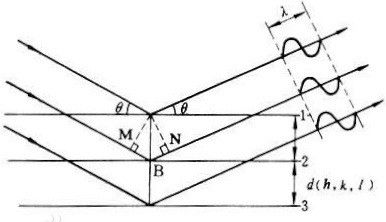
\includegraphics[width=0.4\linewidth]{Chp16_20.PNG}
\caption{2.10图}
\end{figure}

根据光波干涉加强的条件,即相干光波之间光程差相隔$k\lambda$,即$d(sin\theta+sin\theta)=k\lambda$,化简得$2dsin\varphi=k\lambda,k=1,2,3...$。
\section{计算题}
\exercise

\solve
(1)由光栅方程$(a+b)sin\varphi=\pm k\lambda$;

当$\varphi=30°,k=1$时;

解得$a+b=10^{-6}\mathrm{m}$;

所以光栅常数为$10^{-6}\mathrm{m}$。

(2)由题意得:$\lambda=(1\pm5\% ) \lambda_0$;
\quad 代入光栅方程得:$(a+b)sin(\varphi\pm\frac{1}{2}\Delta\theta)=\pm k(1\pm5\%)\lambda_0$;

解得:$\theta_{min}=arcsin\frac{95\%\lambda_0}{a+b}=28.359°$;

$\theta_{max}=arcsin\frac{105\%\lambda_0}{a+b}=31.668°$;

得:$\Delta\theta\in[-1.641°,1.668°]$.

\exercise

\solve
根据单缝衍射条纹的暗纹条件,即$asin\varphi=\pm2k\frac{\lambda}{2}$;

中央亮纹的宽度为两侧第一级暗条纹的距离,此时$k=1$;

又由于几何关系:$sin\varphi\approx tan\varphi=\frac{x}{f}$;

当$2x=1.0\mathrm{cm}$时,$a_1=4.8\times10^{-5}\mathrm{m}$;
当$2x=1.5\mathrm{cm}$时,$a_2=3.2\times10^{-5}\mathrm{m}$;

即缝宽由$4.8\times10^{-5}\mathrm{m}$变为$3.2\times10^{-5}\mathrm{m}$。

\exercise

\solve
光栅衍射明条纹的条件为:$dsin\varphi=\pm2k\frac{\lambda}{2}$;

对光$\lambda_1$:$dsin\varphi=k_1\lambda_1$;

对光$\lambda_2$:$dsin\varphi=k_2\lambda_2$;

所以$k_1\lambda_1=k_2\lambda_2$,即$k_1=1.5k_2$;

当$k_1=3,k_2=2$时,两条光波第一次重合;

当$k_1'=6,k_2'=4$时,两条光波第二次重合

即$dsin\varphi=k_1'\lambda_1$;

得$d=\frac{k_1'\lambda_1}{sin\varphi}=3.05\times10^{-6}\mathrm{m}$。

\exercise

\solve
设最小分辨角为$\delta_\varphi$;

代入数据得:
\[
\delta_\varphi\approx\frac{1\mathrm{m}}{645\times10^{3}\mathrm{m}}=1.55\times10^{-6}\mathrm{rad}
\]
由最小分辨角公式$\delta_\varphi=\varphi_0\approx1.22\frac{\lambda}{D}$得:
\[
D=0.394\mathrm{m}
\]

\chapter{波动光学3(偏振)}
\section{选择题}
\exercise B

\solve 由马吕斯定律知,线偏光透过检偏器时的光强$I=I_0\mathrm{cos}^2\theta$,故光强先增加,后减小至0。

\exercise D

\solve A:部分偏振光可以看作是线偏光和自然光的合成,而自然光的光振动沿任意方向都有分布,正确;

B:部分偏振光的自然光分量透过旋转的偏振片永远不会使光强降为0,正确;

C:自然偏振光和线偏光均可以分解为两个相互正交的、无相位关系的线偏光,正确;

D:部分偏振光中的自然光分量在经过偏振片时光强一定会减小,错误,选D。

\exercise C

\solve 从偏振度的定义来看,图中两个方向偏振的光的标记数量得越均匀,则偏振度越小。其中C图两个方向偏振的光的标记数量相等,是自然光,故偏振度为0,偏振度最小,选C。

\exercise C

\solve 如果入射光是部分偏振光,则在偏振光旋转的时候,部分偏振光的线偏振光部分的光强会变化,而自然偏振光部分不会变化,叠加起来导致出射光强对偏振片转动有变化但没有消光,满足条件;

如果是椭圆偏振光,则可根据椭圆的对称轴将偏振光分解为正交的两个分量$I_1\leqslant I_2$,总光强$I_0=I_1+I_2$,如图\ref{4}所示。

\begin{figure}[htbp]
	\centering
	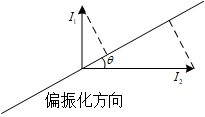
\includegraphics[scale=0.9]{Chp17_4.jpg}
	\caption{题4\ 示意图}
	\label{4}
\end{figure}

其中在经过偏振片后,透过两线偏光光强分别为$I_1'=I_1\mathrm{sin}^2\theta$,$I_2'=I_2\mathrm{cos}^2\theta$。而$I_1',I_2'$原本d的相位差为$\frac{\pi}{2}$或$\frac{3\pi}{2}$,在有些时候,当偏振方向使得矢量在相反方向分解时,有附加相位差$\pi$,故总的相位差仍可化为$\Delta \varphi=\frac{\pi}{2},\frac{3\pi}{2}$。而两线偏光在同一偏振面内,故合成的是线偏光,光强为$I=I_1'+I_2'+2\mathrm{cos}\Delta \varphi\sqrt{I_1'I_2'}$,代入上述关系,得$I=I_1\mathrm{sin}^2\theta+I_2\mathrm{cos}^2\theta=I_1+(I_2-I_1)\mathrm{cos}^2\theta$。当$I_1\not= I_2$时,$I$会随$\theta$变化,且$I_2-I_1>0$,光强不会变为0,不会消光,这种椭圆偏振光满足条件;而当$I_1=I_2$时,即圆偏光,$I=I_1=I_2=\frac{1}{2}I_0$,光强与偏振片角度无关,即光强不变化,故圆偏光一定不满足条件。

如果入射光是线偏光,则当偏振化方向与偏振方向垂直时会消光,不满足条件。

由以上讨论对选项进行检查:A,B:入射光是部分偏振光或是非圆偏光的椭圆偏振光时,可以满足条件,故两者都错;C:入射光是圆偏光时,偏振光旋转不可能使光强发生变化,故不可能是圆偏光,正确;D:旋转偏振片可以使线偏光消光,错误。

\exercise A

\solve 在光经过偏振片后,光的强度减为原来的一般,而光的偏振方向相同,仍然满足干涉条件,故在屏上仍有干涉条纹,但光强减为原来的一半,选A。

\exercise B

\solve 由书中介绍,可以得知自然光入射到两种介质界面上时,反射光一般是部分偏振光,在入射角为布儒斯特角时反射光为线偏光。故ACD正确,B错误。

\exercise B

\solve 由于自然光是以布儒斯特角从空气入射玻璃,故1光是线偏振光,2光是部分偏振光;而2光从玻璃入射空气时,也是以布儒斯特角入射,故反射光3是线偏振光,且光矢量方向垂直于入射面,选B。

\exercise C

\solve 由书中对o光和e光的介绍,知o光在晶体中的波阵面是球面,e光在晶体中的波阵面是旋转椭球面,选C。

\exercise C

\solve 见题4对椭圆偏振光透过偏振片的光强的推导,有当椭圆偏振光为圆偏光时,透过的线偏光的光强为$I=\frac{1}{2}I_0$,是原来光强的一半。故选C。

\exercise A

\solve 自然光可以沿1/4波片的光轴方向分解为两个光强相等的正交分量,但没有固定的相位关系,故在通过波片后,虽然某一方向的相位增加了$\frac{\pi}{2}$,但两分量的相位差仍然没有固定关系,但两分量的光强度不变,所以出射光仍然是自然光,选A。

\section{填空题}

\exercise 起偏方向$\quad$起偏器$\quad$检偏器

\solve 由书中定义可得。

\exercise 平行于入射面

\solve 已知以布儒斯特角入射的光线,其反射光只能是垂直于入射面的;而由于这束偏振光没有反射的部分,故该偏振光没有垂直于入射面的分量,故该偏振光的光矢量振动方向为平行于入射面。

\exercise $\frac{\sqrt{2}}{2}A$

\solve 将振幅沿偏振光方向分解,沿偏振方向的振幅为$A'=A\mathrm{cos}45^{\mathrm{o}}=\frac{\sqrt{2}}{2}A$,故透过偏振片的光振幅为$\frac{\sqrt{2}}{2}A$。

\exercise $60^{\mathrm{o}}$

\solve 自然光透过第一个偏振片后光强变为$I'=\frac{1}{2}I_0$,变为线偏光,再经过第二个偏振片后光强变为$I=I'\mathrm{cos}^2\theta=\frac{1}{2}\mathrm{cos}^2\theta I_0$,其中$\theta$为两偏振片的夹角。又知$I=\frac{1}{8}I_0$,故有$\frac{1}{2}\mathrm{cos}^2\theta=\frac{1}{8}$,取$0\leqslant\theta\leqslant 90^{\mathrm{o}}$,有$\theta=60^{\mathrm{o}}$。

\exercise 线偏光$\quad$垂直于入射面$\quad$部分偏振光

\solve 由书中对布儒斯特角的介绍可得。

\exercise $\mathrm{arctan}\frac{n_2}{n_1}$

\solve 入射角为$i_B$(布儒斯特角)时,折射角为$\gamma=\frac{\pi}{2}-i_B$。又由折射关系,知$n_1\mathrm{sin}i_B=n_2\mathrm{sin}\gamma=n_2\mathrm{cos}i_B$,故$\mathrm{tan}i_B=\frac{n_2}{n_1}$,有$i_B=\mathrm{arctan}\frac{n_2}{n_1}$。

\exercise $\frac{1}{2}I$

\solve 由题4对椭圆偏振光中特殊情况圆偏光的分析可得。

\exercise o$\quad$e

由书中对双折射现象的介绍可得。

\exercise $5\times 10^{-6}\mathrm{m}$

\solve 由o光和e光在材料中不同的折射率,得材料中o光和e光的光程差为$\Delta=d|n_o-n_e|$,其中$d$为材料的厚度;当$\Delta=\frac{\lambda}{4}+k\lambda,k=0,1,2,\cdots$时,可以变为1/4波片。为使$d$最小,取$k=0$,得$d_{\mathrm{min}}=\frac{\lambda}{4|n_e-n_o|}=5\times 10^{-6}\mathrm{m}$。

\exercise 在光路中添加1/2波片

\solve 将右旋椭圆偏振光沿波片的光轴分解为正交的两个振动分量,假设分解如图\ref{fig:17_20}中方向所示。

\begin{figure}[htbp]
	\centering
	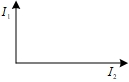
\includegraphics[scale=0.9]{Chp17_20.jpg}
	\caption{题20\ 示意图}
	\label{fig:17_20}
\end{figure}

由于偏振光右旋,故$I_2$方向的偏振超前$I_1$方向$\Delta \varphi\leqslant\frac{\pi}{2}$;在通过半波片后,$I_2$方向的偏振超前$I_1$方向$\Delta \varphi\pm\pi$,均可等效为$\Delta \varphi'=\Delta \varphi-\pi$,其中$-\frac{\pi}{2}\leqslant\Delta \varphi'\leqslant0$,可理解为$I_1$超前$I_2$的相位为$-\Delta \varphi'=\pi-\Delta \varphi$,则方向变为右旋。故可以通过加1/2波片使椭圆偏振光从右旋变成左旋。

\section{计算题}
\exercise 

\solve 设部分偏振光的自然光部分的光强为$I_1$,线偏光部分的光强为$I_2$。在偏振片移动到透射光强最大位置时,偏振化方向与线偏光相同,则透射光强为$I_{\mathrm max}=\frac{1}{2}I_1+I_2$;当偏振片旋转$60^{\mathrm{o}}$时,透射光强为$I=\frac{1}{2}I_1+I_2\mathrm{cos}^260^{\mathrm{o}}$。由题中所给关系$I=\frac{1}{2}I_{\mathrm max}$,解得$I_1:I_2=1:1$。

\exercise $45^{\mathrm{o}}$

\solve 设第二个偏振片和第一个偏振片的夹角为$\theta$,则第二个偏振片和第三个偏振片的夹角为$90^{\mathrm{o}}-\theta$。则有透射光光强为$I=\frac{1}{2}I_0\mathrm{cos}^2\theta\mathrm{cos}^2(90^{\mathrm{o}}-\theta)=\frac{1}{2}I_0\mathrm{cos}^2\theta\mathrm{sin}^2\theta=\frac{1}{8}I_0\mathrm{sin}^22\theta$。则当$\theta=45^{\mathrm{o}}$时,光强最大。

\exercise $I'=\frac{5}{8}I_0$$\quad$$I''=\frac{5}{32}I_0$

\solve 入射光为强度相等的线偏振光和自然偏振光混合而成,故线偏光部分强度为$I_1=\frac{1}{2}I_0$,自然光部分强度为$I_2=\frac{1}{2}I_0$。在该光经过第一个偏振片时,光强变为$I'=I_1\mathrm{cos}^2 30^{\mathrm{o}}+\frac{1}{2}I_2=\frac{5}{8}I_0$,为线偏光。再经过第二个偏振片,光强变为$I''=I'\mathrm{cos}^2 60^{\mathrm{o}}=\frac{5}{32}I_0$。

\exercise $1.28\mathrm{\mu m}$

\solve 设晶片的厚度为$d$。光的分解和叠加情况如图\ref{24}所示。

\begin{figure}[htbp]
	\centering
	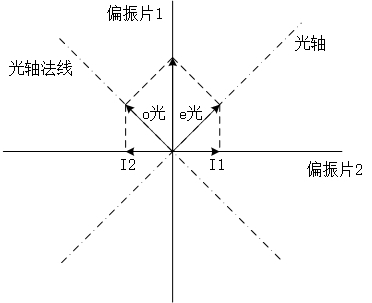
\includegraphics[scale=0.6]{Chp17_24.jpg}
	\caption{题24\ 示意图}
	\label{fig:17_24}
\end{figure}

从图\ref{fig:17_24}中可以看出,在自然光经过偏振片1后,变为线偏光;在经过方解石晶片后被分解为o光和e光,并且由于其在晶片中的运动速度不同,产生了一部分光程差;再经过偏振片2,o光和e光均被分解到偏振片2的方向($I_1,I_2$)。可以看出,其参考方向相反,则在干涉叠加的时候又附加光程差$\frac{\lambda}{2}$。故$I_1,I_2$之间总光程差为$\delta=d|n_o-n_e|+\frac{\lambda}{2}$。而当$\delta=n\lambda,n=1,2,\cdots$时,光达到相长干涉,光通过系统达到极大。则计算得满足条件的$d=\frac{\lambda}{|n_o-n_e|}n-\frac{\lambda}{2|n_o-n_e|}=3.488n-1.744(\mathrm{\mu m})$。

当$n=3$时,$d=8.720 \mathrm{\mu m}<10 \mathrm{\mu m}$;
当$n=4$时,$d=12.208 \mathrm{\mu m}>10 \mathrm{\mu m}$。
故$d$取$8.720 \mathrm{\mu m}$,
应至少磨去$\Delta d=10-8.720=1.28 \mathrm{\mu m}$(保留三位有效数字)。

\chapter{量子物理基础}

\section{选择题}
\exercise A

\solve 考察绝对黑体的定义。能够全部吸收各种波长的辐射能而完全不发生反射和透射的物体称为绝对黑体。故选A。

\exercise C

\solve 斯特藩-玻尔兹曼定律:$M(T)=\sigma T^4$,其中T是黑体自身温度,与环境温度无关。由于$T_A=T_B$,所以$M_A=M_B$。

\exercise C

\solve 电子绕核运动角动量的大小有表达式$L=\sqrt{l(l+1)h}$。其中$l<n$,为角量子数。%?

题给$3.464h$,即$2\sqrt{3}h$,令$\sqrt{l(l+1)h}=2\sqrt{3}h$,解得$l=3$。故选C。

\exercise A

\solve 产生光电效应的光子需满足能量大于逸出功的条件。即$h\frac{c}{\lambda}\ge eU_0$,整理得$\lambda \le\frac{hc}{eU_0}$。故选A。

\exercise D

\solve A选项,\alpha 粒子散射实验验证了原子的核式结构,与光的性质无关;B选项,辐射电磁波反应体现光的波动性;C选项,电子束的衍射图样说明了物质的波动性;D选项,光电效应反应光的粒子性,康普顿效应也能体现光的粒子性。故选D。

\exercise B

\solve 根据维恩位移定律:$\lambda_mT=b$,加热前后波长之比$\frac{\lambda_1}{\lambda_2}=\frac{6}{5}$,故$\frac{T_1}{T_2}=\frac{5}{6}$。结合斯特藩-玻尔兹曼定律:$M(T)=\sigma T^4$,所以$\frac{M_1}{M_2}=(\frac{5}{6})^4\approx\frac{1}{2}$。故选B。

\exercise C

\solve $p=\sqrt{2mE_k}=\frac{h}{\lambda}$,代入数据,得德布罗意波长$\lambda=2.0\times10^{-14}$,故选C

\exercise D

\solve 微观粒子具有的明显的波动性,以致它的某些成对物理量不可能同时具有确定的量值。$\Delta x\cdot \Delta p_x\ge h$就描述就描述了位置与动量不能同时准确确定。故选D。

\exercise C

\solve 由不确定关系,平均寿命$\Delta t\approx\frac{h}{2\pi\times2\Delta E}=\frac{6.626\times10^{-34}}{2\pi\times2\times9\times1.6\times10^{-19}}=3.5\times10^{-23}$,注意此处为约化普朗克常量,故选C。

\exercise A

\solve $h\lambda=mv,v=\frac{h}{m\lambda}\approx900\mathrm{m/s}$,故选A。

\section{填空题}

\exercise 1416

\solve $T=(\frac{M}{\sigma})^\frac{1}{4}$,解得$T=1416K$。本题注意单位统一。

\exercise 频率$\quad$绝对黑体幅射光的频率处在可见光范围内。

\solve 书中定义可知。

\exercise 半导体$\quad$绝缘体

\solve 被束缚的电子要成为自由电子或者空穴,就必须获得足够能量从价带跃迁到导带,这个能量的最小值就是禁带宽度。因此禁带宽度与导电难易程度负相关,半导体远的禁带宽度小于绝缘体。

\exercise 自发$\quad$不是$\quad$受激$\quad$是

\solve 书中定义可知。

\exercise $\sqrt{\frac{h}{2m(\nu-\nu_0)}}$

\solve $h\nu-h\nu_0=E_k=\frac{p^2}{2m}=\frac{h^2}{2m\lambda^2}$,解得$\lambda=\sqrt{\frac{h}{2m(\nu-\nu_0)}}$

\exercise 9

\solve $n=3$时;$l=0,1,2;m_l=0,\pm1,\pm2$。又由于$l<n,m_l\le l$,排列组合得$n=3$对应的电子态数目有1+3+5=9种。

\exercise 0$\quad\frac{h\nu}{c^2}$

\solve 由于光子是以光速运动,故静止质量必然为零;$E=mc^2=h\nu$,故光子的相对论质量为$\frac{h\nu}{c^2}$。

\exercise $1.45\times10^{-10}m\quad6.6\times10^{-29}m$

\solve$\lambda=\frac{h}{p}=\frac{h}{mv},\sqrt{\bar{v}^2}=\sqrt{\frac{3RT}{M}}=2735m/s$

所以$\lambda_1=\frac{6.6\times10^{-34}}{1.67\times10^{-27}}\times2735=1.45\times10^{-10}\mathrm{m}$
$\lambda_2=\frac{6.6\times10^{-34}}{1x10^{-3}}\times1\times10^{-2}=6.6\times10^{-29}\mathrm{m}$

\exercise 错误$\quad$该波函数不能满足在$x=0$连续且满足归一化条件

\solve 波函数需要连续且满足归一化条件。若该定态波函数满足连续条件,则$\psi_0=0,A=0$,故$  \int_{-\infty}^{+\infty}|\psi(x)|^2\cdot dx=0$,不满足归一化条件。故无法同时满足连续与归一化,所以是错误的。

\exercise 0.225

\solve 由势阱中粒子能级公式
\begin{gather*}
	E_n=n^2\frac{h^2}{8mL^2}\\
	E_3-E_1=h\frac{c}{\lambda}
\end{gather*}
解得$L=0.225\mathrm{nm}$。

\section{解答题}

\exercise

\solve 利用维恩位移定律以及斯忒藩-玻尔兹曼定律$T\lambda_m=b$,$M_B(T)=\sigma T^4$

太阳表面温度 
\begin{center}$T_1=\frac{B}{\lambda_{m1}}=\frac{2.898\times10^{-3}}{510\times10^{-9}}=5682\mathrm{K}$\end{center}
辐出度
\begin{center}$\qquad\qquad M_{B1}=\sigma T_1^4=5.9\times10^7\mathrm{W/m^2}$\end{center}
北极星表面温度
\begin{center}$\quad T_2=\frac{b}{\lambda_{m2}}=\frac{2.898\times10^{-3}}{350\times10^{-9}}=8280\mathrm{K}$\end{center}
辐出度
\begin{center}$\qquad\qquad M_{B2}=\sigma T_2^4=2.7\times10^7\mathrm{W/m^2}$\end{center}

\exercise

\solve (1)由$\nu=\frac{c}{\lambda}1.5\times10^{15}\mathrm{s^{-1}}$
\begin{equation}\nonumber
\begin{split}
E_k&=h\nu-W_0\\
&=6.3\mathrm{eV}-4.2\mathrm{eV}\\
&=2.0\mathrm{eV}\\
\end{split}
\end{equation}
(2)由$eU_0=E_k$,$U_0=2.0\mathrm{V}$。

(3)由$h\nu_0=W_0$
\begin{gather*}
	\nu_0=1.014\times10^{25} \mathrm{s^{-1}}
	\lambda=\frac{c}{\nu_0}=296\mathrm{nm} 
\end{gather*}

\exercise

\solve 
\[ |\psi(x)|^2=\frac{2}{a}\sin{\frac{\pi x}{a}}^2=\frac{1}{a}(1-\cos{\frac{2\pi x}{a}}) \quad (0\le x \le a) \]
$\therefore \cos{\frac{2\pi x}{a}}=-1$时,概率最大\\
即
\[ \frac{2\pi x}{a}=\pi \]
\[ x=\frac{a}{2} \]
	
\exercise

\solve 设自由电子静$m_0$,它与光子碰撞后吸收光子,然后以速度$v_2$运动,电子碰前速度为$v_1$,碰前电子和光子的夹角为$\theta_1$,碰后为$\theta_2$,如图\ref{Chp18_24}

\begin{figure}[htbp]
	\centering
	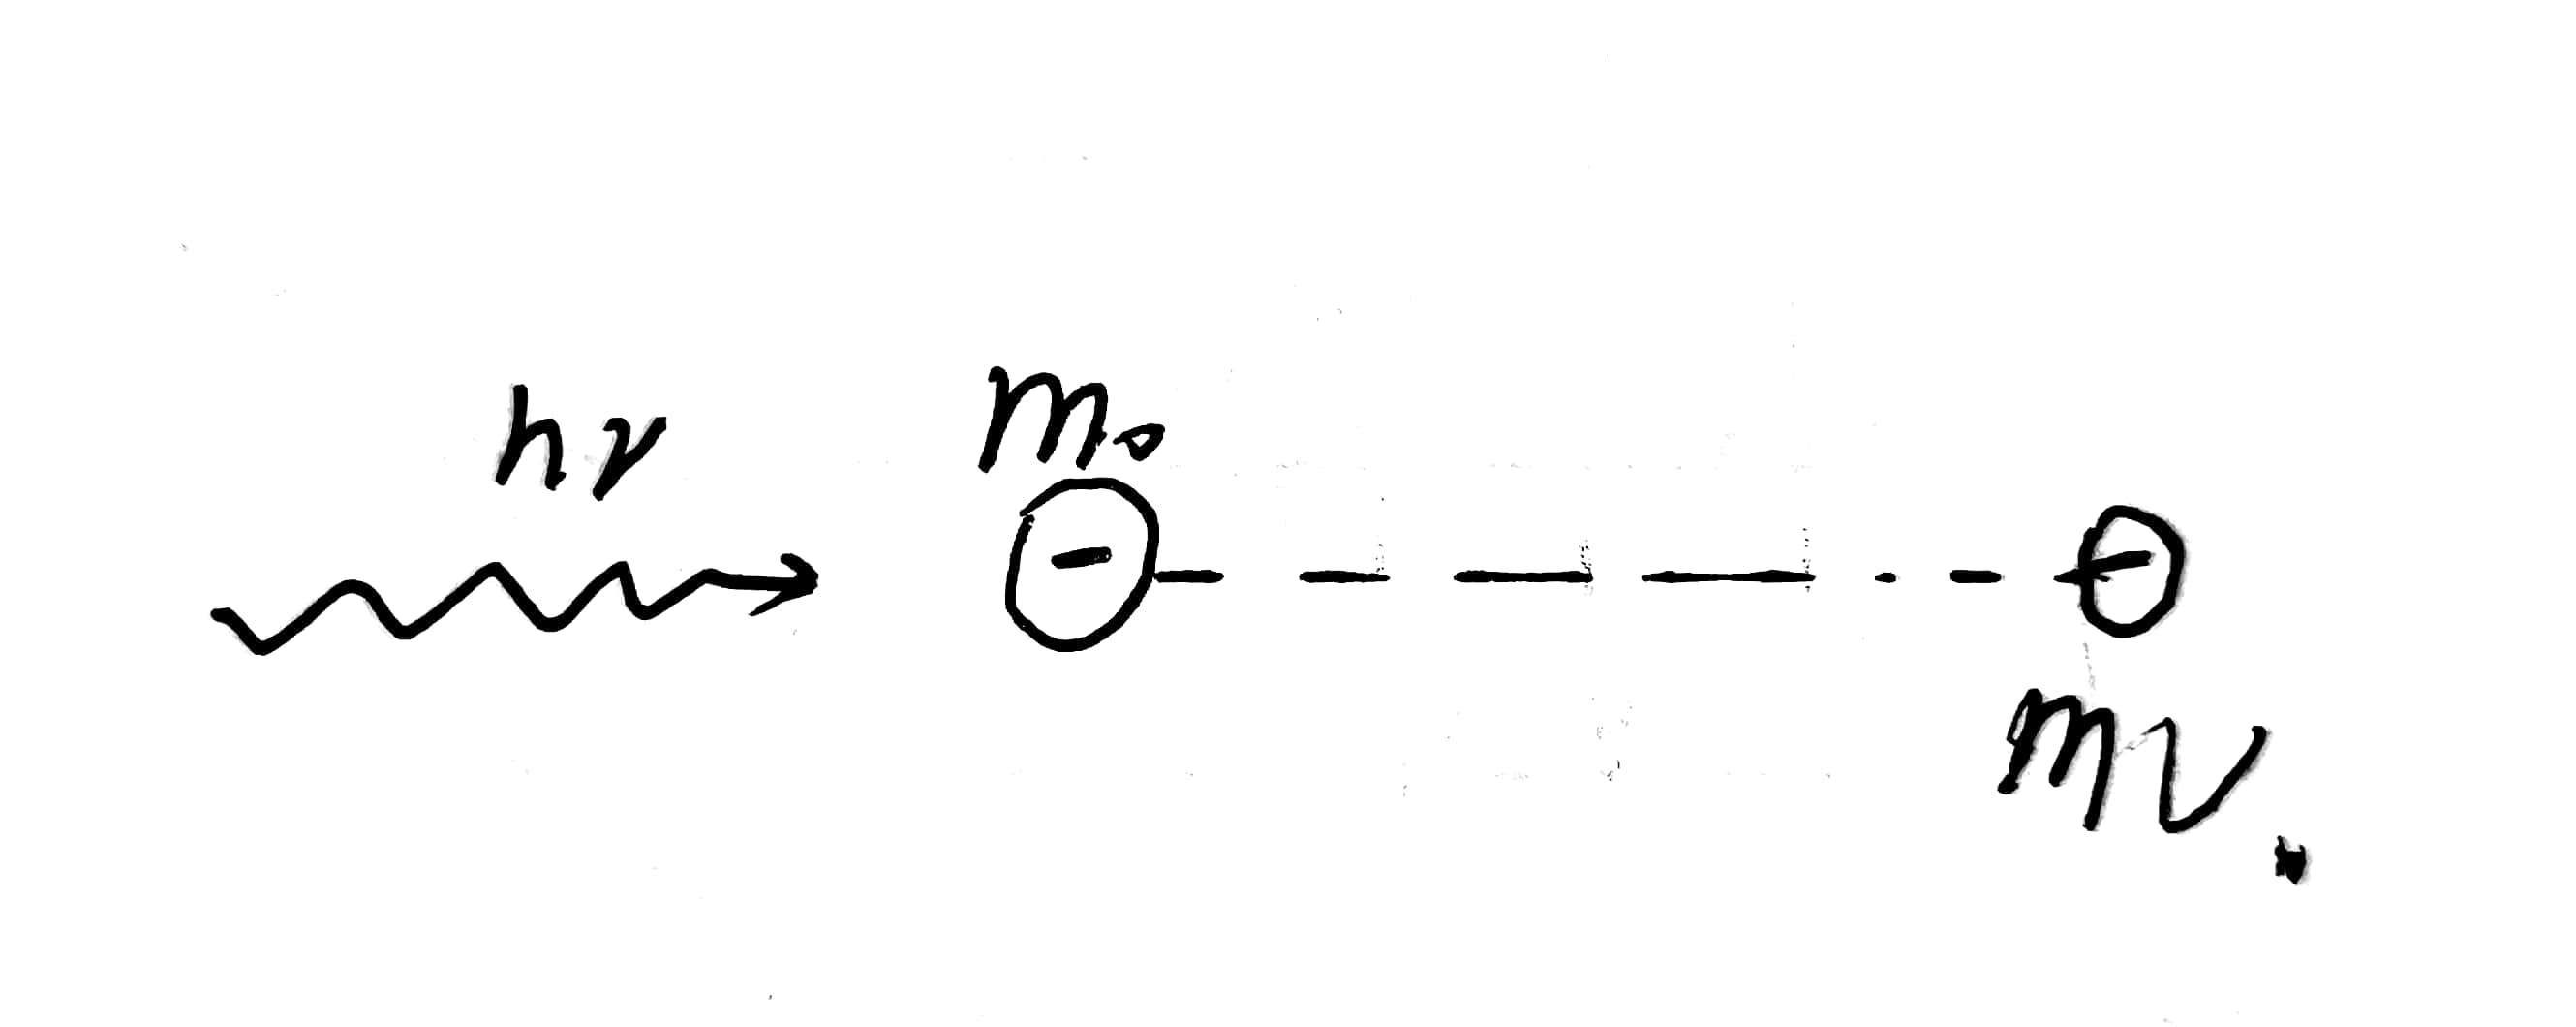
\includegraphics[width=0.6 \textwidth]{Chp18_24.jpg}
	\caption{题24图}
	\label{Chp18_24}
\end{figure}
由动量守恒
\[ x:\frac{h\nu}{c}+m_1v_1\cos\theta_1=\frac{m_0v_2}{\sqrt{1-\frac{v_2}{c}^2}}\cos\theta_2 \]
\[ y:m_1v_1\sin\theta_1=\frac{m_0v_2}{\sqrt{1-\frac{v_2}{c}^2}}\sin\theta_2 \]
解得
\[ v_2=c\sqrt{\frac{h^2\nu^2+m_1^2v_1^2c^2+2h\nu m_1v_1\cos\theta_1}{m_0^2c^4+h^2\nu^2+m_1^2v_1^2c^2+2h\nu m_1v_1\cos\theta_1}} \]

若能量全部转移,由能量守恒
\[ h\nu+m_1c^2=\frac{m_0}{\sqrt{1-\frac{v_2'}{c}^2}}\cdot c^2 \]
解得
\[v_2'=\frac{c\sqrt{h^2\nu^2+(m_1^2-m_0^2)c^4+2h\nu m_1c^2}}{h\nu+m_1c^2}  \]
由于$v_2\neq v_2'$,说明光子不可能把能量全部转移给电子。

\end{document}
